\documentclass[sigconf,review,anonymous]{acmart}

\usepackage{booktabs}
\usepackage{tabularx}
\usepackage{array}
\usepackage{xspace}
\usepackage{enumitem}
\usepackage{listings}
\usepackage{balance}
\usepackage{xcolor}
\usepackage{xurl}
\usepackage{graphicx}
\usepackage{tikz}
\usetikzlibrary{arrows.meta,positioning,calc}

\definecolor{modelblue}{RGB}{37,99,235}
\definecolor{modelorange}{RGB}{194,65,12}
\definecolor{modelgreen}{RGB}{21,128,61}
\definecolor{finalcolor}{RGB}{37,99,235}
\definecolor{chaincolor}{RGB}{21,128,61}
\definecolor{tracecolor}{RGB}{194,65,12}

\newcommand{\benchmark}{ReachabilityBench\xspace}
\newcommand{\taskname}{reachability\xspace}
\newcommand{\true}{\textsc{True}\xspace}
\newcommand{\false}{\textsc{False}\xspace}
\newcommand{\researchq}[1]{\textbf{RQ#1}}
\newcommand{\datasetroot}{\texttt{src/code\_generation}\xspace}
\newcommand{\inferenceroot}{\texttt{src/inference}\xspace}
\newcommand{\analysisroot}{\texttt{src/analysis}\xspace}
\newcommand{\secref}[1]{\hyperref[#1]{Section~\ref*{#1}}}
\newcommand{\figref}[1]{\hyperref[#1]{Figure~\ref*{#1}}}
\newcommand{\figpanelref}[2]{\hyperref[#1]{Figure~\ref*{#1}#2}}
\newcommand{\tabref}[1]{\hyperref[#1]{Table~\ref*{#1}}}
\newcommand{\TODO}[1]{\textcolor{red}{TODO: #1}}
\newcommand{\redtodo}[1]{\TODO{#1}}
\providecommand{\Description}[1]{}
% Avoid stretched bibliography spacing and line-number output interference.
\newcommand{\BIBdecl}{\nolinenumbers\raggedbottom}
% Shared visual conventions for the manuscript's diagrams and result plots.
\usepackage{pgfplots}
\usepgfplotslibrary{groupplots}
\pgfplotsset{compat=1.18}
\definecolor{rbInk}{HTML}{263238}
\definecolor{rbMuted}{HTML}{667078}
\definecolor{rbRule}{HTML}{BAC1C6}
\definecolor{rbPaper}{HTML}{F5F7F8}
\definecolor{modelblue}{HTML}{0072B2}
\definecolor{modelorange}{HTML}{D55E00}
\tikzset{
  rb diagram/.style={font=\sffamily\footnotesize, text=rbInk, >=Latex},
  rb method/.style={draw=rbInk, fill=white, line width=0.65pt,
    rounded corners=1pt, minimum height=0.52cm, minimum width=0.85cm,
    inner sep=3pt, align=center, font=\sffamily\footnotesize},
  rb edge/.style={->, draw=rbInk, line width=0.7pt},
  rb optional edge/.style={rb edge, dashed},
  rb annotation/.style={font=\sffamily\scriptsize, text=rbMuted,
    fill=white, inner sep=2pt, align=center},
  rb block/.style={draw=rbRule, fill=rbPaper, line width=0.65pt,
    rounded corners=1pt, text width=2.35cm, minimum height=1.25cm,
    inner sep=5pt, align=center, font=\sffamily\footnotesize},
  rb heading/.style={font=\sffamily\footnotesize\bfseries, text=rbInk},
  rb note/.style={font=\sffamily\scriptsize, text=rbMuted, align=center},
  rb query/.style={draw=rbRule, fill=rbPaper, line width=0.55pt,
    rounded corners=1pt, inner sep=5pt, align=left,
    font=\sffamily\footnotesize}
}
\pgfplotsset{
  rb score axis/.style={
    width=8.1cm, height=4.9cm, ymin=0, ymax=100,
    ytick={0,25,50,75,100}, axis lines=left,
    axis line style={draw=rbRule, line width=0.6pt, -},
    tick style={draw=rbRule}, tick align=outside,
    ymajorgrids=true, grid style={draw=rbRule!55, line width=0.3pt},
    font=\sffamily\footnotesize,
    tick label style={font=\sffamily\scriptsize, text=rbMuted},
    label style={font=\sffamily\footnotesize, text=rbInk},
    title style={font=\sffamily\footnotesize\bfseries, text=rbInk},
    ylabel={Correctness (\%)}, scaled ticks=false,
    legend style={draw=none, fill=none, font=\sffamily\scriptsize,
      /tikz/every even column/.append style={column sep=9pt}},
    legend cell align=left, clip=false
  },
  rb gemma/.style={color=modelorange, mark=*, mark size=1.8pt, line width=0.9pt},
  rb qwen/.style={color=modelblue, mark=square*, mark size=1.8pt, line width=0.9pt},
  rb path/.style={dashed, mark options={solid}},
  rb answer/.style={solid}
}



\hypersetup{
  colorlinks=true,
  linkcolor=ACMBlue,
  citecolor=ACMBlue,
  urlcolor=ACMBlue
}

\settopmatter{printacmref=false}
\renewcommand\footnotetextcopyrightpermission[1]{}

\acmConference[ICSE '27]{International Conference on Software Engineering}{Conference Date TBD}{Location TBD}
\acmYear{2027}
\copyrightyear{2027}
\acmDOI{}
\acmISBN{}

\title{Benchmarking Large Language Models on Controlled Java Reachability Tasks}

\author{Anonymous Author(s)}
\affiliation{%
  \institution{Anonymous Institution}
  \city{Anonymous City}
  \country{Anonymous Country}
}

\begin{document}

\begin{abstract}
Large language models (LLMs) are increasingly used as software-engineering assistants, yet it remains difficult to tell when a correct answer reflects faithful program reasoning. We study this question through generated Java tasks that isolate two forms of program comprehension: control-flow reachability, where a model must decide whether one method can call another directly or indirectly, and data-flow tracing, where the same benchmark design can require following values across calls, parameters, and local state. The benchmark exposes graph family, context size, source-target depth, syntactic distractors, and requested reasoning budget as explicit experimental factors, and it evaluates both final Boolean answers and the traces that justify them. In the current control-flow study, three reasoning-capable models are evaluated on a common slice of 108,000 samples over contexts of 100, 250, and 500 methods, depths 1--25, and requested budgets from 512 to 16,384 tokens. The results show that final-answer accuracy substantially overstates reasoning quality: Gemma reaches 90.1\% final accuracy but only 57.2\% exact-chain accuracy, GPT-OSS reaches 79.0\% and 36.3\%, and Qwen reaches 89.1\% and 66.4\%. Budget helps, but only model-specifically: Qwen converts budget into large final and chain gains, Gemma saturates early, and GPT-OSS improves final answers faster than trace fidelity. These findings suggest that reasoning-budget evaluations for software engineering should report path-level evidence, not only final labels.

\end{abstract}

\keywords{large language models, software engineering benchmark, program comprehension, reachability, control-flow, condition-aware execution}

\maketitle

\section{Introduction}

LLMs are now widely used in software engineering, particularly to assist developers with tasks such as program understanding, debugging, code review, and code generation. To evaluate their capabilities on these tasks, many benchmarks have been proposed with the objective of reproducing problems that are close to those encountered by developers.

However, these benchmarks mainly provide a global measure of whether a model can solve a specific task. They can therefore indicate whether a model performs well in a given scenario, but they make it more difficult to diagnose the reasons behind its success or failure. A single task can involve several skills at the same time, which makes it difficult to identify precisely which elements cause difficulties for the model. For example, a model may understand a program by partially relying on semantic information present in method or variable names, while its performance may decrease when this information is removed. A correct or incorrect answer alone is not sufficient to highlight this type of behavior.

In this work, we propose \benchmark, a Java benchmark whose objective is not to replace existing benchmarks, but to provide an evaluation framework that allows a more fine-grained analysis of model capabilities. \benchmark focuses on reachability problems between methods. Given a source method and a target method, the model must determine whether the target can be reached from the source through a sequence of calls.

The Java code used in the benchmark is automatically generated from call graphs. This provides an executable-graph oracle and the expected answer for each question. The model returns a JSON object with a Boolean final answer and an ordered sequence of explored methods. The evaluator scores these outputs independently, accepting any path order justified by executable edges rather than requiring one canonical traversal.

\benchmark provides two families of tasks. The first, \emph{unguarded reachability}, considers programs in which calls are executed whenever they are reached because they are outside control structures. The second, \emph{condition-aware reachability}, introduces calls inside conditions that can make some calls executable or non-executable. The model must then reason about the data flow to determine which conditions are satisfied and, as a consequence, which method calls are actually executed. This second task therefore distinguishes what is visible in the source code from what happens during program execution.

Through this approach, \benchmark aims to provide a more controlled and diagnostic evaluation of LLMs on program-understanding tasks. It makes it possible to study model behavior according to specific factors rather than limiting the evaluation to whether the final answer is correct.
This paper makes three contributions:
\begin{itemize}[leftmargin=*]
    \item a configurable benchmark that generates Java reachability problems together with executable call graphs and oracle labels;
    \item an empirical study of \texttt{[N\_MODELS]}, supported by an artifact containing the complete generation and evaluation pipeline.
\end{itemize}

\section{Background and Motivation}
\label{sec:background}

\subsection{LLM Benchmarks for Software Engineering}

LLM benchmarks for software engineering fall into several loose families. One family evaluates code synthesis from natural-language specifications. HumanEval~\cite{chen2021codex} and MBPP~\cite{austin2021program} are the familiar examples: a model completes short Python functions, and unit tests decide whether the result works. APPS~\cite{hendrycks2021apps} raises the difficulty with larger programming-contest problems and richer tests. These benchmarks remain useful because they are cheap to run and easy to compare, yet their main signal is generation rather than analysis of an existing program.

A second family tries to make the setting more realistic and less vulnerable to contamination. LiveCodeBench~\cite{jain2024livecodebench} uses time-aware problem collection and includes scenarios beyond simple generation, such as repair and execution-oriented tasks. BigCodeBench~\cite{zhuo2024bigcodebench} puts more weight on complex instructions and library use, closer to everyday API programming. Its core signal still comes from producing or manipulating code under test-based evaluation.

A third family targets broader software-engineering work. CodeXGLUE~\cite{lu2021codexglue} covers code search, summarization, translation, defect detection, and other code-intelligence problems. Defects4J~\cite{just2014defects4j} provides real Java bugs for repair and testing research. SWE-bench~\cite{jimenez2024swebench} asks whether a model or agent can resolve real GitHub issues by editing repositories and passing tests. These tasks are closer to maintenance, but diagnosis becomes harder. A failure may reflect weak issue understanding, poor localization, an incorrect edit, missing tool use, or insufficient program reasoning.

\tabref{tab:benchmark-positioning} places \benchmark relative to these families. The distinction is granularity. \benchmark does not ask the model to synthesize behavior or repair a repository. It isolates a program-comprehension judgment that is small enough to control but still requires structured reasoning over code.

\begin{table*}[t]
\centering
\caption{Position of \benchmark relative to common LLM benchmarks for software engineering.}
\label{tab:benchmark-positioning}
\begin{tabularx}{\textwidth}{p{0.17\textwidth}p{0.20\textwidth}p{0.20\textwidth}p{0.17\textwidth}X}
\toprule
Benchmark & Task & Typical oracle & Granularity & Reachability signal \\
\midrule
HumanEval / MBPP & Function synthesis & Unit tests & Single function & Indirect \\
APPS & Algorithmic programming & Test cases & Full program & Indirect \\
LiveCodeBench & Live coding scenarios & Test cases / scenarios & Problem level & Indirect \\
BigCodeBench & API-rich generation & Test cases & Function / program & Indirect \\
CodeXGLUE & Code intelligence suite & Task-specific labels & Mixed & Partial \\
Defects4J & Bug repair / bug testing & Regression tests & Real Java bugs & Indirect \\
SWE-bench & Issue resolution & Repository tests & Real repositories & Indirect \\
\benchmark & Method-to-method reachability & Generated oracle and trace & Controlled Java class & Direct \\
\bottomrule
\end{tabularx}
\end{table*}


\subsection{Reachability as a Program-Comprehension Task}

Reachability is a basic concept in program analysis. At method level, it asks whether execution starting from one method can eventually invoke another. The same relation appears in call-graph construction, impact analysis, security auditing, dead-code detection, testing strategies, debugging, and program understanding. Traditional static-analysis research has studied how to build call graphs soundly and scalably~\cite{grove2001framework,tip2000scalable}. In safety-critical settings, LLMs are a poor substitute for those analyses. At the same time, developer-facing assistants increasingly answer questions that look like lightweight program analysis.

For an LLM, reachability is deceptively simple. A shallow case may reduce to spotting a direct call. A deeper case requires following several method definitions. A negative case adds another burden: the target may appear in the file, yet remain outside the subgraph reachable from the source. With a tree-shaped call structure, sibling branches may have to be checked before the target can be found or ruled out. Comments, variables, parameters, loops, and conditionals add surface code for the model to filter while leaving the underlying call relation unchanged.

That combination makes reachability a useful diagnostic task. The expected output can include a Boolean answer and a trace. Evaluation can then distinguish cases that test-pass metrics often merge together: the right answer for the wrong reason, a partial path, a hallucinated call edge, skipped intermediate methods, or an early stop.

\subsection{Why a Controlled Synthetic Benchmark?}

Real projects are essential for external validity. Generated programs serve a different purpose: they make a specific capability measurable. In \benchmark, generation gives direct control over context size, target depth, graph shape, and syntactic distractors. Ground truth comes from construction, rather than from brittle manual labeling. The resulting task is not a substitute for real-repository benchmarks; it is an interpretable lens on one ability that broader benchmarks implicitly require.

The implementation generates Java programs organized around method-call trees. Each benchmark case contains the generated class, the prompt context, reachability questions, expected chains, and configuration metadata. Positive questions use reachable source-target pairs; negative questions use targets outside the source's reachable subgraph. The experimental factors include context size, call depth, comments, variables, loops, conditionals, and parameters. Together they support questions about scaling, robustness, and reasoning quality.

\subsection{Terminology}

In the terminology used here, the \emph{source method} is where traversal begins, and the \emph{target method} is the queried destination. A \emph{reachable} target can be invoked directly or indirectly from the source through method calls. A \emph{trace} is the ordered list of methods visited or reported by the model. A \emph{chain} is the expected source-to-target path for reachable cases; for unreachable cases, it is the expected explored path defined by the benchmark oracle. The \emph{distance} or \emph{depth} is the absolute value of the stored question distance. Positive distances denote reachable questions, and negative distances denote unreachable questions.

\section{\benchmark Design}
\label{sec:benchmark-design}

\begin{figure*}[t]
\centering
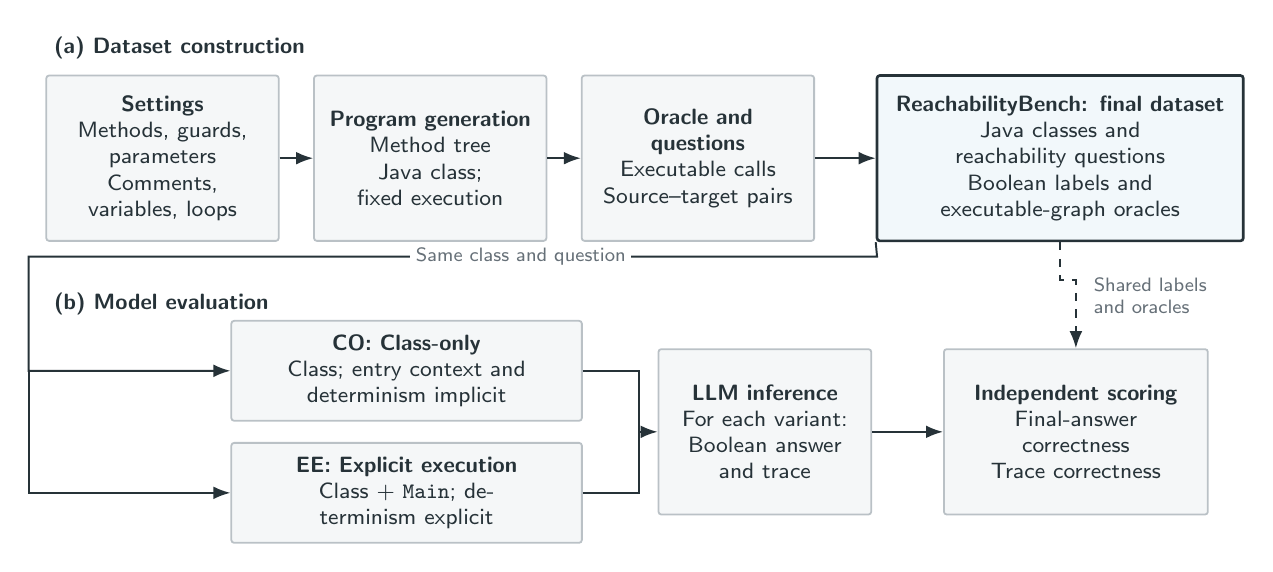
\begin{tikzpicture}[rb diagram,
  pipeline block/.style={rb block, text width=2.6cm, minimum height=2.1cm},
  pipeline prompt/.style={rb block, text width=4.1cm, minimum height=1cm},
  pipeline oracle/.style={rb edge, dashed}]

\node[rb heading, anchor=west] at (0,1.4) {(a) Dataset construction};
\node[pipeline block] (settings) at (1.5,0)
  {\textbf{Settings}\\Methods, guards, parameters\\Comments, variables, loops};
\node[pipeline block] (java) at (4.9,0)
  {\textbf{Program generation}\\Method tree\\Java class; fixed execution};
\node[pipeline block] (questions) at (8.3,0)
  {\textbf{Oracle and questions}\\Executable calls\\Source--target pairs};
\node[pipeline block, text width=4.3cm, draw=rbInk, line width=0.95pt,
  fill=modelblue!5] (dataset) at (12.9,0)
  {\textbf{\benchmark: final dataset}\\Java classes and reachability questions\\Boolean labels and executable-graph oracles};
\foreach \from/\to in {settings/java,java/questions,questions/dataset}
  \draw[rb edge] (\from.east) -- (\to.west);

\node[rb heading, anchor=west] at (0,-1.85) {(b) Model evaluation};
\node[pipeline prompt] (co) at (4.6,-2.7)
  {\textbf{CO: Class-only}\\Class; entry context and determinism implicit};
\node[pipeline prompt] (ee) at (4.6,-4.25)
  {\textbf{EE: Explicit execution}\\Class + \texttt{Main}; determinism explicit};
\node[pipeline block, text width=2.35cm] (model) at (9.15,-3.475)
  {\textbf{LLM inference}\\For each variant:\\Boolean answer and trace};
\node[pipeline block, text width=3cm] (scoring) at (13.1,-3.475)
  {\textbf{Independent scoring}\\Final-answer correctness\\Trace correctness};

% Only the class and question enter either model prompt.
\draw[rb edge] (dataset.south west) -- (10.575,-1.25)
  -- (-0.2,-1.25) -- (-0.2,-2.7) -- (co.west);
\node[rb annotation] at (6.05,-1.25) {Same class and question};
\draw[rb edge] (-0.2,-2.7) -- (-0.2,-4.25) -- (ee.west);
\draw[rb edge] (co.east) -- (7.55,-2.7) -- (7.55,-3.475) -- (model.west);
\draw[rb edge, -] (ee.east) -- (7.55,-4.25) -- (7.55,-3.475);
\draw[rb edge] (model.east) -- (scoring.west);

% Labels and executable graphs are reserved for evaluation.
\draw[pipeline oracle] (dataset.south) -- (12.9,-1.55)
  -- (13.1,-1.55) -- (scoring.north);
\node[rb annotation, anchor=west, align=left] at (13.25,-1.75)
  {Shared labels\\and oracles};
\end{tikzpicture}
\caption{Construction and evaluation of \benchmark. The construction algorithm produces the final dataset. CO and EE present the same classes and questions with different execution information. Labels and executable-graph oracles are used only for scoring the returned answer and trace.}
\Description{The construction algorithm generates Java classes, records executable calls and selects reachability questions to form ReachabilityBench. The same class and question feed either a Class-only prompt or an Explicit execution prompt with Main and deterministic-execution instructions. Model answers and traces are scored separately against the shared labels and executable-graph oracles, which are not supplied to the model.}
\label{fig:pipeline}
\end{figure*}


\subsection{From a Call Graph to a Reachability Question}

\benchmark starts from a call graph rather than from Java code. The benchmark first generates an ordered graph, then converts each node into a Java method and each edge into a method call. Once the program has been generated, it selects a source method $s$ and a target method $t$. The question asks whether an execution starting from $s$ can reach $t$ through direct or indirect calls.

We represent one benchmark instance with the tuple
\[
    (P, s, t, f, y, \tau, m),
\]
where $P$ is the generated Java program and $f$ identifies the task family. The oracle label $y$ is \true{} when $t$ is executable from $s$, and \false{} otherwise. The oracle trace $\tau$ contains the sequence of methods expected for the question. Finally, $m$ stores the generation parameters and the properties of the graph.

The model receives the complete Java class together with the source and target methods. It must return a JSON object containing two fields:
\begin{itemize}[leftmargin=*]
    \item \texttt{final\_answer}, which contains the Boolean reachability answer; and
    \item \texttt{trace}, which contains the ordered list of methods followed from the source.
\end{itemize}
These two fields are evaluated separately. The final answer shows whether the model reaches the correct decision, while the trace provides information about how it followed the program structure.

Figure~\ref{fig:pipeline} summarizes the complete process. The same generated program is used to build the question, the prompt, and the oracle. After inference, the output is parsed and compared with this oracle. This common origin limits inconsistencies between the program shown to the model and the information used for evaluation.

\subsection{Generating the Call Graph}

The current benchmark uses ordered acyclic trees. This structure allows us to create direct and indirect calls, several branches, and targets that are present in the class but unreachable from the selected source. The order between the children of a node is also important because it defines the order of calls inside the corresponding Java method.

The tree is generated breadth-first under a fixed method budget. Let $u$ be the node currently expanded, and let $L(u)$ and $R(u)$ be its left and right children. When the remaining budget is sufficient, the generator first adds both children:
\[
    u \rightarrow L(u), \qquad u \rightarrow R(u).
\]
It can then add two children below $L(u)$. These additions are sampled independently:
\[
    X_{LL}(u) \sim \mathrm{Bernoulli}(p),
    \qquad
    X_{LR}(u) \sim \mathrm{Bernoulli}(p).
\]
If $X_{LL}(u)=1$, the generator adds $L(u) \rightarrow L(L(u))$. If $X_{LR}(u)=1$, it adds $L(u) \rightarrow R(L(u))$. Figure~\ref{fig:local-tree-rule} shows this local expansion.

\begin{figure}[t]
\centering
\resizebox{\columnwidth}{!}{%
\begin{tikzpicture}[
    >=Latex,
    x=1cm,
    y=1cm,
    method/.style={rb method, minimum width=1.35cm},
    det/.style={rb edge},
    opt/.style={rb optional edge},
    note/.style={font=\scriptsize, align=center}
]
\node[method] (u) at (0,0) {$u$};
\node[method] (l) at (-1.4,-1.0) {$L(u)$};
\node[method] (r) at (1.4,-1.0) {$R(u)$};
\node[method] (ll) at (-2.2,-2.0) {$L(L(u))$};
\node[method] (lr) at (-0.6,-2.0) {$R(L(u))$};
\draw[det] (u) -- node[note, above left] {always} (l);
\draw[det] (u) -- node[note, above right] {always} (r);
\draw[opt] (l) -- node[note, left] {$X_{LL}(u)$} (ll);
\draw[opt] (l) -- node[note, right] {$X_{LR}(u)$} (lr);
\node[rb panel title, text width=4.2cm] at (0,-2.75) {Optional edges are sampled independently with probability $p$.};
\end{tikzpicture}
}
\caption{Local rule used to expand the generated tree. The fixed edges create the main structure, while the optional edges add branches.}
\Description{A node u has deterministic left and right children. The left child has two optional children, each controlled by an independent Bernoulli variable.}
\label{fig:local-tree-rule}
\end{figure}

With this rule, $L(u)$ receives zero, one, or two optional children with probabilities $(1-p)^2$, $2p(1-p)$, and $p^2$. Increasing $p$ increases the number of branches and therefore the number of possible negative questions. The final level can be truncated when the method budget is reached. All labels and traces are computed from this final tree. We use $p=0.65$ to generate enough positive and negative questions; the sensitivity to this value remains to be studied.

\subsection{Generating the Java Program}

After the tree has been generated, each node becomes one Java method. An edge $u \rightarrow v$ inserts a call to $v$ inside the body of $u$. Calls are inserted in the order defined by the tree. In contrast, method declarations are shuffled in the final class. The position of a method in the source file therefore does not reveal the order in which it is executed.

The generator can also add comments, local variables, parameters, loops, and different declaration orders. These elements change the code that is presented to the model, but they do not change reachability unless they are used in a generated condition. In the current benchmark, calls used to define reachability are not placed inside loops.

\subsection{Introducing Runtime Conditions}

The two task families are produced from the same general pipeline, but they differ in the way calls are inserted. In unguarded reachability, every generated call is placed directly in the method body. If execution reaches this statement, the call is executed.

In condition-aware reachability, some calls are placed inside generated \texttt{if} statements. The generator fixes the values used in the conditions and can therefore determine whether each call is executed. The model must reproduce this evaluation from the Java code. It is not sufficient to identify that a call is visible in the method body.

This distinction creates two call graphs. The syntactic graph $G_{\mathit{syn}}$ contains all calls visible in the source code. The executable graph $G_{\mathit{exec}}$ contains only calls whose conditions allow them to execute. The two graphs are equal for unguarded programs. For condition-aware programs, $G_{\mathit{exec}}$ can exclude edges from $G_{\mathit{syn}}$. When a model follows one of these excluded edges, we classify the behavior as \emph{syntactic-call bias}.

\subsection{Building the Oracle Trace}

The oracle is computed after the complete Java program has been generated. It follows executable calls in their source order, starting from the method given in the question. For a positive question, the trace stops when the target is reached for the first time. For a negative question, it continues until the complete region reachable from the source has been explored. Condition-aware traces use $G_{\mathit{exec}}$ and ignore calls whose conditions are false.

This convention means that the canonical trace is not always a shortest path. Execution can visit an earlier sibling branch before reaching the target. Similarly, a negative trace must cover all methods reachable from the source. A model can therefore find a valid path to the target and return the correct Boolean answer without reproducing the complete canonical trace.

\begin{figure}[t]
\centering
\resizebox{\columnwidth}{!}{%
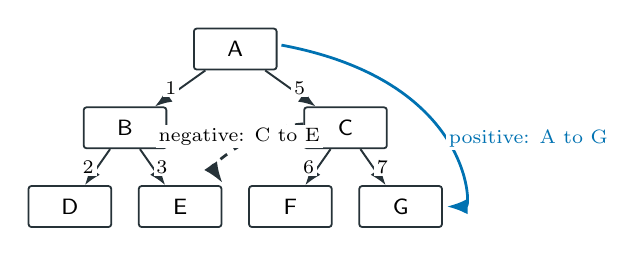
\begin{tikzpicture}[
    >=Latex,
    method/.style={rb method, minimum width=1.05cm},
    edge/.style={rb edge},
    visit/.style={font=\scriptsize, fill=white, inner sep=1pt}
]
\node[method] (a) at (0,0) {A};
\node[method] (b) at (-1.4,-1.0) {B};
\node[method] (c) at (1.4,-1.0) {C};
\node[method] (d) at (-2.1,-2.0) {D};
\node[method] (e) at (-0.7,-2.0) {E};
\node[method] (f) at (0.7,-2.0) {F};
\node[method] (g) at (2.1,-2.0) {G};
\draw[edge] (a) -- node[visit, left] {1} (b);
\draw[edge] (a) -- node[visit, right] {5} (c);
\draw[edge] (b) -- node[visit, left] {2} (d);
\draw[edge] (b) -- node[visit, right] {3} (e);
\draw[edge] (c) -- node[visit, left] {6} (f);
\draw[edge] (c) -- node[visit, right] {7} (g);
\draw[->, line width=1pt, modelblue] ($(a.east)+(0.05,0.05)$) .. controls (3.0,-0.4) and (3.0,-2.0) .. node[visit, right] {positive: A to G} ($(g.east)+(0.05,0)$);
\draw[rb optional edge, line width=1pt] ($(c.west)+(0,0.05)$) .. controls (0.2,-1.0) and (-0.3,-1.5) .. node[visit, above] {negative: C to E} ($(e.north east)+(0,0.03)$);
\end{tikzpicture}
}
\caption{Canonical traversal of a generated call graph. A positive trace includes the calls executed before the target, while a negative trace covers all methods reachable from the source.}
\Description{A tree-shaped call graph with ordered traversal labels and two example reachability queries.}
\label{fig:canonical-traversal}
\end{figure}

We represent the required exploration with a signed canonical trace length. Let $\tau=\langle m_0,\ldots,m_k\rangle$, where $m_0=s$. A positive question has length $+k$, and $m_k=t$. A negative question has length $-k$, where $k$ is the number of steps required to explore the source-reachable region. The sign indicates whether the question is positive or negative, while the magnitude represents the amount of exploration. It is not a shortest-path distance.

\subsection{Configuration and Validation}

The final dataset contains \texttt{[N\_INSTANCES]} questions with context sizes \texttt{[CONTEXT\_SIZES]} and canonical trace lengths \texttt{[DISTANCE\_RANGE]}. Positive and negative labels are balanced at the retained trace lengths. Each released instance contains the Java program, source and target methods, label, canonical trace, task family, class size, graph properties, and generated-condition metadata.

Before an instance is included, the validator compiles its Java class and checks that the generated calls correspond to the intended tree. It then recomputes reachability in $G_{\mathit{exec}}$, verifies the outcome of each generated condition, and checks the canonical trace. As a result, the oracle is validated against the program that is shown to the model rather than only against the state of the generator.

\section{Experimental Methodology}
\label{sec:methodology}

This section describes how \benchmark is evaluated once a dataset release has been frozen. The benchmark definition in \secref{sec:benchmark-design} fixes the meaning of an instance, the syntactic and executable call graphs, and the canonical trace. The methodology below focuses on the experimental protocol: which generated instances are retained, how models are served, how prompts are constructed, how outputs are parsed, and how scores are analyzed. The final dataset parameters are still open and are therefore recorded as controlled placeholders rather than fixed claims.

\subsection{Dataset Release}

The evaluation unit is one validated source--target query over one generated Java class. Each retained query has an oracle Boolean label, an oracle canonical trace, and metadata describing the generation factors. The frozen release will contain \texttt{[N\_CLASSES]} generated classes and \texttt{[N\_INSTANCES]} queries. It will also record the final context-size grid, trace-length range, question count per retained trace length, guard settings, parameter settings, and random seeds as \texttt{[DATASET\_CONFIGURATION]}.

The dataset is produced by the benchmark generator rather than sampled from repositories. In the current generator, the default full sweep is restricted to Java and tree-shaped programs. The generator materializes each context as a directory containing the Java class, the prompt context, reachability questions, oracle chains, method names, and configuration metadata. For each requested trace length, it selects positive and negative queries in balanced pairs when both are available; depths that cannot supply enough valid pairs contribute fewer instances or are omitted from the retained release.

\begin{table*}[t]
\centering
\caption{Detailed configuration of the evaluation set. Both task families use the same generation grid.}
\label{tab:dataset-spec}
\scriptsize
\begin{tabularx}{\textwidth}{p{0.22\textwidth}p{0.24\textwidth}X}
\toprule
Category & Parameter & Value \\
\midrule
Dataset size & Java classes & 1,232 per task family \\
& Questions & 46,656 per task family \\
& Question polarity & 23,328 reachable and 23,328 unreachable \\
\midrule
Graph generation & Target class size & $\{100,250,500\}$ methods \\
& Absolute source--target distance & $\{1,4,7,10,13,16,19,22,25\}$ \\
& Local tree structure & Three trees of depth three; two calls per function \\
& Helper-call probability & 0.2 in total \\
\midrule
Generated code & Comments & $\{0,1\}$ \\
& Variables, loops, and parameters & $\{0,1,2\}$ \\
& Conditionals or guards & $\{0,1,3,5\}$ \\
\midrule
Factorial design & Code configurations & $3\times2\times3\times3\times4\times3=648$ \\
& Questions per distance and configuration & Four reachable and four unreachable \\
\midrule
Task semantics & Unguarded & All generated direct calls contribute to reachability \\
& Condition-aware & Only calls whose generated guards evaluate to true contribute to reachability \\
\bottomrule
\end{tabularx}
\end{table*}


\subsection{Experimental Factors}

The primary factors are task family, signed canonical trace length, generated class size, query polarity, and model configuration. For condition-aware instances, we additionally analyze guard-related metadata such as the number of generated \texttt{if} statements and whether predicted transitions use calls that are syntactically visible but not executable. Other code-surface settings, including comments, local variables, loops, method parameters, and declaration order, are retained as metadata and used only when they are part of the frozen dataset configuration.

The unguarded and condition-aware families are compared at the level of matched factor distributions. Unless the final release explicitly pairs the same abstract graph and query across families, we do not treat family comparisons as paired observations.

\subsection{Model Serving and Inference}

We evaluate \texttt{[N\_MODELS]} locally served LLM configurations. A configuration is not just a checkpoint name: it includes the serving backend, precision, tensor parallelism, context limit, decoding parameters, output budget, and whether the deployment exposes a reasoning-budget control. Reporting at the configuration level is necessary because the same checkpoint can behave differently under different serving and budget settings.

\begin{table*}[!t]
\centering
\caption{Model configurations used in the evaluation. Checkpoint and serving information will be added after the final configurations are frozen.}
\label{tab:models}
\scriptsize
\begin{tabularx}{\textwidth}{p{0.25\textwidth}p{0.22\textwidth}p{0.22\textwidth}X}
\toprule
Configuration & Inference mode & Budget metadata & Reproducibility metadata \\
\midrule
\texttt{[MODEL\_CONFIG\_1]} & \texttt{[MODE\_1]} & \texttt{[BUDGET\_CONTROL\_1]} & checkpoint, size, context, license and source, serving settings \\
\texttt{[MODEL\_CONFIG\_2]} & \texttt{[MODE\_2]} & \texttt{[BUDGET\_CONTROL\_2]} & checkpoint, size, context, license and source, serving settings \\
\texttt{[MODEL\_CONFIG\_3]} & \texttt{[MODE\_3]} & \texttt{[BUDGET\_CONTROL\_3]} & checkpoint, size, context, license and source, serving settings \\
\texttt{[MODEL\_CONFIG\_4]} & \texttt{[MODE\_4]} & \texttt{[BUDGET\_CONTROL\_4]} & checkpoint, size, context, license and source, serving settings \\
\texttt{[MODEL\_CONFIG\_5]} & \texttt{[MODE\_5]} & \texttt{[BUDGET\_CONTROL\_5]} & checkpoint, size, context, license and source, serving settings \\
\bottomrule
\end{tabularx}
\end{table*}


The intended serving stack uses vLLM on the Jean Zay supercomputer operated by IDRIS~\cite{cnrs2024jeanzay}. The inference runner starts a local OpenAI-compatible vLLM server, resolves model-context and GPU-memory settings, reads generated experiment directories, and writes one result file per directory. Final serving values, including backend version, GPU type, precision, tensor-parallel size, concurrency, context limit, and memory-utilization settings, are recorded as \texttt{[SERVING\_CONFIGURATION]}.

For reasoning-budget experiments, the runner supports an explicit sweep over requested reasoning budgets. When thinking mode is enabled, it first requests a bounded reasoning segment, then continues from that segment with a separate final-answer budget. When thinking mode is disabled or unavailable, the same task is run as a direct answer generation with the configured answer budget. The final paper will report budget effects only for configurations where the serving stack actually exposes and enforces the requested reasoning-budget control.

\subsection{Prompting}

Each prompt contains the generated Java class, the source method, the target method, and the required JSON output schema. It does not expose oracle labels, oracle traces, generator metadata, or evaluator internals. The required object has two fields: \texttt{final\_answer}, a Boolean reachability prediction, and \texttt{trace}, an ordered list of method names.

The prompt template differs only where the task family requires it. The unguarded template asks the model to follow method calls from the queried source. The condition-aware template additionally instructs the model to account for generated values and guards when deciding whether a visible call executes. The complete prompt templates and any illustrative examples are frozen before inference and included in the anonymized artifact as \texttt{[PROMPT\_ARTIFACT]}.

\subsection{Output Parsing}

Model outputs are parsed after inference by a deterministic parser. The parser extracts the final valid JSON object when extra text appears before or after the answer. A case is marked \texttt{NO\_RESPONSE} when no valid object can be decoded, when \texttt{final\_answer} is missing or cannot be interpreted as a Boolean, or when generation ends before an extractable answer appears.

The \texttt{trace} field is expected to be a JSON list of method names. Normalization is deliberately limited: it may handle unambiguous formatting variants, but it must not invent method names or repair semantically invalid traces. All primary accuracy metrics use strict scoring, so \texttt{NO\_RESPONSE} counts as incorrect and is also reported as a separate failure mode.

\subsection{Metrics}

\begin{table*}[t]
\centering
\caption{Evaluation metrics used for final answers, traces, and budget behavior.}
\label{tab:metrics}
\begin{tabularx}{\textwidth}{p{0.25\textwidth}X}
\toprule
Metric & Definition \\
\midrule
Final-answer accuracy & Predicted \true/\false matches the oracle label \\
Exact-chain accuracy & Predicted method chain exactly matches the expected oracle chain \\
Trace accuracy & Predicted trace satisfies the stricter trace representation used by the evaluator \\
Trace completeness & Fraction of the expected trace recovered in order \\
Emitted reasoning length & Tokenizer-counted visible reasoning text extracted from the model response; not a runtime consumed-token counter \\
\bottomrule
\end{tabularx}
\end{table*}


The metrics are designed to separate answer correctness from trace behavior. Final-answer accuracy measures the Boolean label only. Exact canonical trace accuracy requires the full predicted trace to match the oracle trace. Trace completeness gives ordered-recall credit for oracle methods recovered in canonical order, starting from the queried source. Graph-valid exploration checks whether predicted transitions are executable and whether the trace satisfies the family-specific stopping condition. Syntactic-call bias is evaluated on condition-aware instances by detecting predicted transitions that follow visible calls excluded from the executable graph by generated guards.

\subsection{Statistical Analysis}

The final analysis reports uncertainty for all primary proportions and bounded trace-completeness scores. The exact confidence-interval procedure is \texttt{[CI\_METHOD]}, and the trace-completeness interval procedure is \texttt{[TRACE\_CI\_METHOD]}. Factor-level analyses use the frozen metadata rather than post-hoc labels inferred from source text.

For the main factor analysis, candidate predictors are task family, signed canonical trace length, class size, query polarity, guard count, model configuration, and selected interactions justified by the research questions. If multiple queries come from the same generated class, the analysis accounts for within-class dependence using \texttt{[DEPENDENCE\_MODEL]}. Model-by-factor breakdowns that are not part of the preregistered analysis plan are treated as exploratory.

\subsection{Baselines and Sanity Checks}

The LLM configurations are the systems under study. Non-LLM baselines are used to calibrate interpretation, not to compete with the oracle.

\begin{itemize}[leftmargin=*]
    \item \textbf{Random-label baseline.} Predicts according to the empirical label distribution and emits a minimal trace, calibrating Boolean accuracy under label balance.
    \item \textbf{Syntactic-call baseline.} Treats every visible call as executable, estimating how far source-level call visibility alone can go.
    \item \textbf{Shortest-executable-path baseline.} Uses the executable graph to answer reachability and emit a shortest path for positive queries, separating semantic reachability from the stricter canonical trace convention.
    \item \textbf{Oracle-traversal sanity check.} Recomputes labels and traces from the validated executable graph and should match the stored oracle by construction.
\end{itemize}

The final set of reported baselines is \texttt{[MAIN\_BASELINES]}. Any implementation-only sanity checks are documented in the artifact rather than treated as experimental systems.

\subsection{Reproducibility}

The anonymized artifact will contain the frozen dataset, generated Java programs, oracle metadata, prompt templates, inference configurations, raw or filtered model outputs when shareable, parser and metric implementations, statistical scripts, and dashboard materials. The review artifact location is \texttt{[ARTIFACT\_URL]}. When model-license or storage constraints prevent sharing raw outputs, the artifact records the restriction and provides parsed outputs sufficient to reproduce the reported tables.

\section{Results}
\label{sec:results}

\subsection{Target Organization of Results}

\begin{itemize}[leftmargin=*]
    \item The final paper should present results in research-question order, not in the order of the currently available scripts.
    \item Proposed narrative:
    \begin{itemize}[leftmargin=*]
        \item overall performance on reachability tasks;
        \item effect of structural factors;
        \item control-flow vs data-flow comparison;
        \item reasoning vs non-reasoning comparison and effect of the requested budget.
    \end{itemize}
    \item Current status:
    \begin{itemize}[leftmargin=*]
        \item the tables and figures below mostly document the preliminary control-flow study;
        \item subsections RQ1 to RQ4 currently remain placeholders for writing and future analysis.
    \end{itemize}
\end{itemize}

\begin{figure*}[t]
\centering
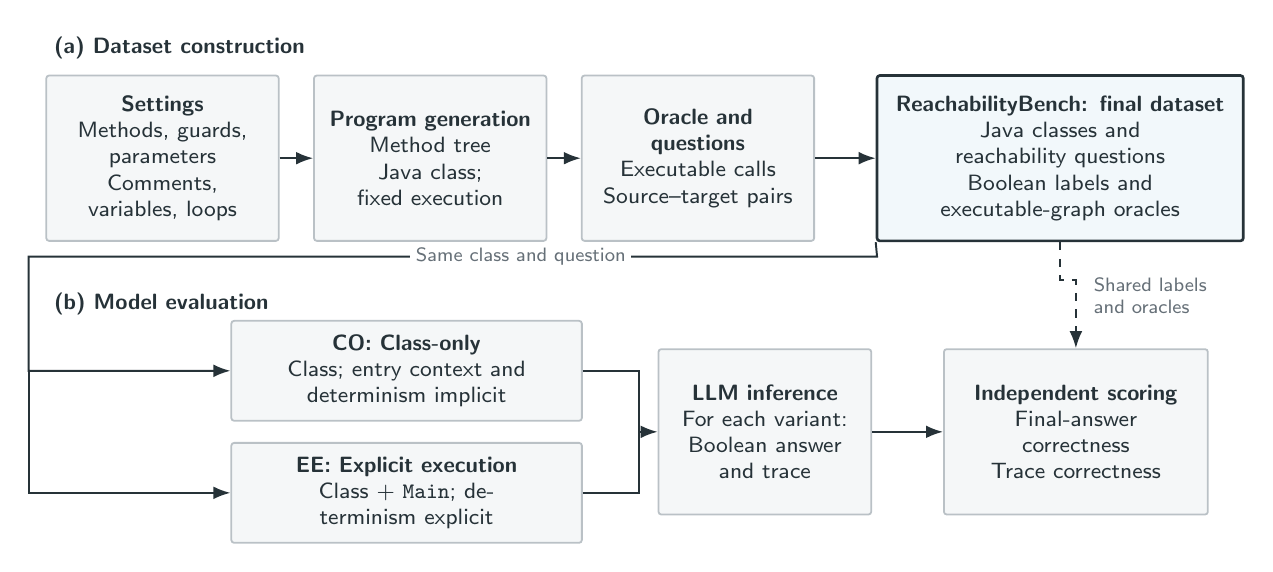
\begin{tikzpicture}[rb diagram,
  pipeline block/.style={rb block, text width=2.6cm, minimum height=2.1cm},
  pipeline prompt/.style={rb block, text width=4.1cm, minimum height=1cm},
  pipeline oracle/.style={rb edge, dashed}]

\node[rb heading, anchor=west] at (0,1.4) {(a) Dataset construction};
\node[pipeline block] (settings) at (1.5,0)
  {\textbf{Settings}\\Methods, guards, parameters\\Comments, variables, loops};
\node[pipeline block] (java) at (4.9,0)
  {\textbf{Program generation}\\Method tree\\Java class; fixed execution};
\node[pipeline block] (questions) at (8.3,0)
  {\textbf{Oracle and questions}\\Executable calls\\Source--target pairs};
\node[pipeline block, text width=4.3cm, draw=rbInk, line width=0.95pt,
  fill=modelblue!5] (dataset) at (12.9,0)
  {\textbf{\benchmark: final dataset}\\Java classes and reachability questions\\Boolean labels and executable-graph oracles};
\foreach \from/\to in {settings/java,java/questions,questions/dataset}
  \draw[rb edge] (\from.east) -- (\to.west);

\node[rb heading, anchor=west] at (0,-1.85) {(b) Model evaluation};
\node[pipeline prompt] (co) at (4.6,-2.7)
  {\textbf{CO: Class-only}\\Class; entry context and determinism implicit};
\node[pipeline prompt] (ee) at (4.6,-4.25)
  {\textbf{EE: Explicit execution}\\Class + \texttt{Main}; determinism explicit};
\node[pipeline block, text width=2.35cm] (model) at (9.15,-3.475)
  {\textbf{LLM inference}\\For each variant:\\Boolean answer and trace};
\node[pipeline block, text width=3cm] (scoring) at (13.1,-3.475)
  {\textbf{Independent scoring}\\Final-answer correctness\\Trace correctness};

% Only the class and question enter either model prompt.
\draw[rb edge] (dataset.south west) -- (10.575,-1.25)
  -- (-0.2,-1.25) -- (-0.2,-2.7) -- (co.west);
\node[rb annotation] at (6.05,-1.25) {Same class and question};
\draw[rb edge] (-0.2,-2.7) -- (-0.2,-4.25) -- (ee.west);
\draw[rb edge] (co.east) -- (7.55,-2.7) -- (7.55,-3.475) -- (model.west);
\draw[rb edge, -] (ee.east) -- (7.55,-4.25) -- (7.55,-3.475);
\draw[rb edge] (model.east) -- (scoring.west);

% Labels and executable graphs are reserved for evaluation.
\draw[pipeline oracle] (dataset.south) -- (12.9,-1.55)
  -- (13.1,-1.55) -- (scoring.north);
\node[rb annotation, anchor=west, align=left] at (13.25,-1.75)
  {Shared labels\\and oracles};
\end{tikzpicture}
\caption{Construction and evaluation of \benchmark. The construction algorithm produces the final dataset. CO and EE present the same classes and questions with different execution information. Labels and executable-graph oracles are used only for scoring the returned answer and trace.}
\Description{The construction algorithm generates Java classes, records executable calls and selects reachability questions to form ReachabilityBench. The same class and question feed either a Class-only prompt or an Explicit execution prompt with Main and deterministic-execution instructions. Model answers and traces are scored separately against the shared labels and executable-graph oracles, which are not supplied to the model.}
\label{fig:pipeline}
\end{figure*}


\subsection{\researchq{1}: Overall Performance on Reachability Tasks}

\begin{itemize}[leftmargin=*]
    \item Present here the final high-level view of model performance.
    \begin{itemize}[leftmargin=*]
        \item control-flow / data-flow comparison;
        \item reasoning / non-reasoning comparison;
        \item final metrics and trace metrics.
    \end{itemize}
\end{itemize}

\subsection{\researchq{2}: Effect of Structural Difficulty Factors}

\begin{itemize}[leftmargin=*]
    \item Group together here the effects of depth, context, branching, and distractors.
    \item Distinguish clearly between:
    \begin{itemize}[leftmargin=*]
        \item factors intrinsic to the control skeleton;
        \item factors that determine whether guarded calls execute in the data-flow family.
    \end{itemize}
\end{itemize}

\subsection{\researchq{3}: Comparison Between Control Flow and Data Flow}

\begin{itemize}[leftmargin=*]
    \item Show what changes when the same reachability question does or does not require reasoning over values.
    \item Look for useful contrastive cases:
    \begin{itemize}[leftmargin=*]
        \item control flow reachable but data flow unreachable;
        \item control flow easy but data flow difficult;
        \item effects specific to condition evaluation and guarded calls.
    \end{itemize}
\end{itemize}

\subsection{\researchq{4}: Reasoning Models, Non-Reasoning Models, and Requested Budget}

\begin{itemize}[leftmargin=*]
    \item Compare gaps in level, robustness, and failure types.
    \item Check whether the gains of reasoning models are concentrated mainly:
    \begin{itemize}[leftmargin=*]
        \item on the final answer;
        \item on the structural validity of the trace;
        \item on robustness to difficulty factors.
    \end{itemize}
    \item For reasoning models, compare performance across requested reasoning budgets and identify saturation.
    \item A preliminary result is already visible: the requested reasoning budget helps, but differently across models.
    \item Keep a comparative narrative:
    \begin{itemize}[leftmargin=*]
        \item the strongest model overall;
        \item the model that saturates early;
        \item the model whose final answers improve more than its traces.
    \end{itemize}
    \item Key interpretation: final-answer accuracy alone overestimates reasoning quality.
\end{itemize}

\begin{table*}[t]
\centering
\caption{Condition-aware performance over 46,656 questions per model (\%).}
\label{tab:overall}
\scriptsize
\begin{tabular}{lrrr}
\toprule
Model & Final answer & Path & No response \\
\midrule
Gemma-4-26B-A4B & 84.21 & 55.90 & 2.24 \\
Qwen3.6-35B-A3B & \textbf{87.98} & \textbf{67.43} & \textbf{0.83} \\
\bottomrule
\end{tabular}
\end{table*}


\begin{figure*}[t]
    \centering
    \begin{tikzpicture}[x=1cm,y=1cm]
        \draw[modelblue,line width=1.1pt] (3.75,3.62) -- +(0.38,0); \node[right,font=\scriptsize] at (4.20,3.62) {Gemma};
        \draw[modelorange,line width=1.1pt] (5.60,3.62) -- +(0.38,0); \node[right,font=\scriptsize] at (6.05,3.62) {GPT-OSS};
        \draw[modelgreen,line width=1.1pt] (7.75,3.62) -- +(0.38,0); \node[right,font=\scriptsize] at (8.20,3.62) {Qwen};
        \begin{scope}[xshift=0cm]
        \node[rb panel title] at (2.4,3.15) {Final-answer accuracy};
        \draw[rb axis] (0,0) -- (4.8,0);
        \draw[rb axis] (0,0) -- (0,2.6);
        \draw[rb grid] (0,0.00) -- (4.8,0.00);
        \node[left,font=\scriptsize] at (-0.06,0.00) {60\%};
        \draw[rb grid] (0,0.65) -- (4.8,0.65);
        \node[left,font=\scriptsize] at (-0.06,0.65) {70\%};
        \draw[rb grid] (0,1.30) -- (4.8,1.30);
        \node[left,font=\scriptsize] at (-0.06,1.30) {80\%};
        \draw[rb grid] (0,1.95) -- (4.8,1.95);
        \node[left,font=\scriptsize] at (-0.06,1.95) {90\%};
        \draw[rb grid] (0,2.60) -- (4.8,2.60);
        \node[left,font=\scriptsize] at (-0.06,2.60) {100\%};
        \draw[rb axis] (0.00,0) -- +(0,-0.05);
        \node[below,font=\scriptsize] at (0.00,-0.10) {512};
        \draw[rb axis] (0.96,0) -- +(0,-0.05);
        \node[below,font=\scriptsize] at (0.96,-0.10) {1k};
        \draw[rb axis] (1.92,0) -- +(0,-0.05);
        \node[below,font=\scriptsize] at (1.92,-0.10) {2k};
        \draw[rb axis] (2.88,0) -- +(0,-0.05);
        \node[below,font=\scriptsize] at (2.88,-0.10) {4k};
        \draw[rb axis] (3.84,0) -- +(0,-0.05);
        \node[below,font=\scriptsize] at (3.84,-0.10) {8k};
        \draw[rb axis] (4.80,0) -- +(0,-0.05);
        \node[below,font=\scriptsize] at (4.80,-0.10) {16k};
        \draw[modelblue,line width=1.1pt] (0.000,1.708) -- (0.960,1.926) -- (1.920,1.991) -- (2.880,2.007) -- (3.840,2.058) -- (4.800,2.039);
        \fill[modelblue] (0.000,1.708) circle (1.2pt);
        \fill[modelblue] (0.960,1.926) circle (1.2pt);
        \fill[modelblue] (1.920,1.991) circle (1.2pt);
        \fill[modelblue] (2.880,2.007) circle (1.2pt);
        \fill[modelblue] (3.840,2.058) circle (1.2pt);
        \fill[modelblue] (4.800,2.039) circle (1.2pt);
        \draw[modelorange,line width=1.1pt] (0.000,0.322) -- (0.960,0.710) -- (1.920,1.239) -- (2.880,1.588) -- (3.840,1.751) -- (4.800,1.819);
        \fill[modelorange] (0.000,0.322) circle (1.2pt);
        \fill[modelorange] (0.960,0.710) circle (1.2pt);
        \fill[modelorange] (1.920,1.239) circle (1.2pt);
        \fill[modelorange] (2.880,1.588) circle (1.2pt);
        \fill[modelorange] (3.840,1.751) circle (1.2pt);
        \fill[modelorange] (4.800,1.819) circle (1.2pt);
        \draw[modelgreen,line width=1.1pt] (0.000,0.868) -- (0.960,1.363) -- (1.920,1.825) -- (2.880,2.274) -- (3.840,2.484) -- (4.800,2.531);
        \fill[modelgreen] (0.000,0.868) circle (1.2pt);
        \fill[modelgreen] (0.960,1.363) circle (1.2pt);
        \fill[modelgreen] (1.920,1.825) circle (1.2pt);
        \fill[modelgreen] (2.880,2.274) circle (1.2pt);
        \fill[modelgreen] (3.840,2.484) circle (1.2pt);
        \fill[modelgreen] (4.800,2.531) circle (1.2pt);
        \node[below,font=\scriptsize] at (2.4,-0.48) {Requested budget};
        \end{scope}
        \begin{scope}[xshift=6.45cm]
        \node[rb panel title] at (2.4,3.15) {Exact-chain accuracy};
        \draw[rb axis] (0,0) -- (4.8,0);
        \draw[rb axis] (0,0) -- (0,2.6);
        \draw[rb grid] (0,0.00) -- (4.8,0.00);
        \node[left,font=\scriptsize] at (-0.06,0.00) {20\%};
        \draw[rb grid] (0,0.40) -- (4.8,0.40);
        \node[left,font=\scriptsize] at (-0.06,0.40) {30\%};
        \draw[rb grid] (0,0.80) -- (4.8,0.80);
        \node[left,font=\scriptsize] at (-0.06,0.80) {40\%};
        \draw[rb grid] (0,1.20) -- (4.8,1.20);
        \node[left,font=\scriptsize] at (-0.06,1.20) {50\%};
        \draw[rb grid] (0,1.60) -- (4.8,1.60);
        \node[left,font=\scriptsize] at (-0.06,1.60) {60\%};
        \draw[rb grid] (0,2.00) -- (4.8,2.00);
        \node[left,font=\scriptsize] at (-0.06,2.00) {70\%};
        \draw[rb grid] (0,2.40) -- (4.8,2.40);
        \node[left,font=\scriptsize] at (-0.06,2.40) {80\%};
        \draw[rb axis] (0.00,0) -- +(0,-0.05);
        \node[below,font=\scriptsize] at (0.00,-0.10) {512};
        \draw[rb axis] (0.96,0) -- +(0,-0.05);
        \node[below,font=\scriptsize] at (0.96,-0.10) {1k};
        \draw[rb axis] (1.92,0) -- +(0,-0.05);
        \node[below,font=\scriptsize] at (1.92,-0.10) {2k};
        \draw[rb axis] (2.88,0) -- +(0,-0.05);
        \node[below,font=\scriptsize] at (2.88,-0.10) {4k};
        \draw[rb axis] (3.84,0) -- +(0,-0.05);
        \node[below,font=\scriptsize] at (3.84,-0.10) {8k};
        \draw[rb axis] (4.80,0) -- +(0,-0.05);
        \node[below,font=\scriptsize] at (4.80,-0.10) {16k};
        \draw[modelblue,line width=1.1pt] (0.000,1.323) -- (0.960,1.455) -- (1.920,1.525) -- (2.880,1.531) -- (3.840,1.557) -- (4.800,1.544);
        \fill[modelblue] (0.000,1.323) circle (1.2pt);
        \fill[modelblue] (0.960,1.455) circle (1.2pt);
        \fill[modelblue] (1.920,1.525) circle (1.2pt);
        \fill[modelblue] (2.880,1.531) circle (1.2pt);
        \fill[modelblue] (3.840,1.557) circle (1.2pt);
        \fill[modelblue] (4.800,1.544) circle (1.2pt);
        \draw[modelorange,line width=1.1pt] (0.000,0.057) -- (0.960,0.357) -- (1.920,0.707) -- (2.880,0.860) -- (3.840,0.967) -- (4.800,0.975);
        \fill[modelorange] (0.000,0.057) circle (1.2pt);
        \fill[modelorange] (0.960,0.357) circle (1.2pt);
        \fill[modelorange] (1.920,0.707) circle (1.2pt);
        \fill[modelorange] (2.880,0.860) circle (1.2pt);
        \fill[modelorange] (3.840,0.967) circle (1.2pt);
        \fill[modelorange] (4.800,0.975) circle (1.2pt);
        \draw[modelgreen,line width=1.1pt] (0.000,0.846) -- (0.960,1.313) -- (1.920,1.799) -- (2.880,2.275) -- (3.840,2.446) -- (4.800,2.448);
        \fill[modelgreen] (0.000,0.846) circle (1.2pt);
        \fill[modelgreen] (0.960,1.313) circle (1.2pt);
        \fill[modelgreen] (1.920,1.799) circle (1.2pt);
        \fill[modelgreen] (2.880,2.275) circle (1.2pt);
        \fill[modelgreen] (3.840,2.446) circle (1.2pt);
        \fill[modelgreen] (4.800,2.448) circle (1.2pt);
        \node[below,font=\scriptsize] at (2.4,-0.48) {Requested budget};
        \end{scope}
    \end{tikzpicture}
    \caption{Performance as a function of requested reasoning budget. The two panels separate gains on the final answer from gains on exact chain, which makes saturation and metric-specific behavior visible.}
    \Description{Two LaTeX line charts showing the evolution of final-answer accuracy and exact chain as requested budget increases for Gemma, GPT-OSS, and Qwen.}
    \label{fig:budget-scaling-latex}
\end{figure*}

\begin{table*}[t]
    \centering
    \caption{Effect of requested reasoning budget on the common evaluation slice. Each cell reports weighted accuracy.}
    \label{tab:budget}
    \small
    \begin{tabular}{r rr rr rr}
        \toprule
        & \multicolumn{2}{c}{Gemma} & \multicolumn{2}{c}{GPT-OSS} & \multicolumn{2}{c}{Qwen} \\
        \cmidrule(lr){2-3}\cmidrule(lr){4-5}\cmidrule(lr){6-7}
        Budget & Final & Chain & Final & Chain & Final & Chain \\
        \midrule
        512 & 86.3\% & 53.1\% & 65.0\% & 21.4\% & 73.4\% & 41.1\% \\
        1024 & 89.6\% & 56.4\% & 70.9\% & 28.9\% & 81.0\% & 52.8\% \\
        2048 & 90.6\% & 58.1\% & 79.1\% & 37.7\% & 88.1\% & 65.0\% \\
        4096 & 90.9\% & 58.3\% & 84.4\% & 41.5\% & 95.0\% & 76.9\% \\
        8192 & 91.7\% & 58.9\% & 86.9\% & 44.2\% & 98.2\% & 81.2\% \\
        16384 & 91.4\% & 58.6\% & 88.0\% & 44.4\% & 98.9\% & 81.2\% \\
        \bottomrule
    \end{tabular}
\end{table*}

\begin{table*}[t]
    \centering
    \caption{Marginal gains between consecutive requested reasoning budgets, in percentage points. This table identifies where additional budget stops buying meaningful performance.}
    \label{tab:marginal-budget}
    \small
    \begin{tabular}{lrrrrrr}
        \toprule
        & \multicolumn{2}{c}{Gemma} & \multicolumn{2}{c}{GPT-OSS} & \multicolumn{2}{c}{Qwen} \\
        \cmidrule(lr){2-3}\cmidrule(lr){4-5}\cmidrule(lr){6-7}
        Budget step & Final & Chain & Final & Chain & Final & Chain \\
        \midrule
        512 $\rightarrow$ 1024 & +3.3 & +3.3 & +6.0 & +7.5 & +7.6 & +11.7 \\
        1024 $\rightarrow$ 2048 & +1.0 & +1.7 & +8.2 & +8.8 & +7.1 & +12.2 \\
        2048 $\rightarrow$ 4096 & +0.3 & +0.2 & +5.4 & +3.8 & +6.9 & +11.9 \\
        4096 $\rightarrow$ 8192 & +0.8 & +0.6 & +2.5 & +2.7 & +3.2 & +4.3 \\
        8192 $\rightarrow$ 16384 & -0.3 & -0.3 & +1.1 & +0.2 & +0.7 & +0.0 \\
        \bottomrule
    \end{tabular}
\end{table*}

\begin{table*}[t]
    \centering
    \caption{Availability of tokenizer-counted emitted reasoning tokens in the recomputed CSV summaries. The value counts generated reasoning text extracted between \texttt{R:} and \texttt{A:} with each model's local tokenizer; it is a proxy for emitted reasoning length, not a runtime usage counter.}
    \label{tab:budget-observability}
    \small
    \begin{tabular}{lrrl}
        \toprule
        Model & CSV rows & Proxy rows & Status \\
        \midrule
        Gemma & 450 & 450 & tokenizer-counted \\
        GPT-OSS & 450 & 450 & tokenizer-counted \\
        Qwen & 450 & 450 & tokenizer-counted \\
        \bottomrule
    \end{tabular}
\end{table*}

\begin{table*}[t]
    \centering
    \caption{Tokenizer-counted emitted reasoning tokens by requested budget. Cells report weighted means on the shared slice. The proxy can slightly exceed the requested budget at 512, because it is computed post hoc from \texttt{R:} text extracted with the local tokenizer, whereas the decoding budget is enforced by the serving stack.}
    \label{tab:used-budget-by-requested}
    \small
    \begin{tabular}{lrrrrrr}
        \toprule
        Model & 512 & 1024 & 2048 & 4096 & 8192 & 16384 \\
        \midrule
        Gemma & 514 & 988 & 1790 & 2855 & 3835 & 4468 \\
        GPT-OSS & 503 & 969 & 1737 & 2710 & 3512 & 3870 \\
        Qwen & 516 & 1022 & 1924 & 3137 & 3871 & 3941 \\
        \bottomrule
    \end{tabular}
\end{table*}

\begin{itemize}[leftmargin=*]
    \item Add a short reading of saturation below the figure.
    \item Keep the caveat that the requested reasoning budget is an interface control, not an internal cost.
\end{itemize}

\begin{figure*}[t]
    \centering
    \begin{tikzpicture}[x=0.72cm,y=1cm]
        \begin{scope}[shift={(0,0)}]
        \node[rb panel title] at (2.75,3.13) {Context 100};
        \draw[rb axis] (0,0) -- (5.5,0);
        \draw[rb axis] (0,0) -- (0,2.6);
        \draw[rb grid] (0,0.00) -- (5.5,0.00);
        \node[left,font=\scriptsize] at (-0.05,0.00) {60\%};
        \draw[rb grid] (0,0.65) -- (5.5,0.65);
        \node[left,font=\scriptsize] at (-0.05,0.65) {70\%};
        \draw[rb grid] (0,1.30) -- (5.5,1.30);
        \node[left,font=\scriptsize] at (-0.05,1.30) {80\%};
        \draw[rb grid] (0,1.95) -- (5.5,1.95);
        \node[left,font=\scriptsize] at (-0.05,1.95) {90\%};
        \draw[rb grid] (0,2.60) -- (5.5,2.60);
        \node[left,font=\scriptsize] at (-0.05,2.60) {100\%};
        \draw[rb axis] (0.00,0) -- +(0,-0.05);
        \node[below,font=\scriptsize] at (0.00,-0.10) {1};
        \draw[rb axis] (0.92,0) -- +(0,-0.05);
        \node[below,font=\scriptsize] at (0.92,-0.10) {5};
        \draw[rb axis] (2.06,0) -- +(0,-0.05);
        \node[below,font=\scriptsize] at (2.06,-0.10) {10};
        \draw[rb axis] (3.21,0) -- +(0,-0.05);
        \node[below,font=\scriptsize] at (3.21,-0.10) {15};
        \draw[rb axis] (4.35,0) -- +(0,-0.05);
        \node[below,font=\scriptsize] at (4.35,-0.10) {20};
        \draw[rb axis] (5.50,0) -- +(0,-0.05);
        \node[below,font=\scriptsize] at (5.50,-0.10) {25};
        \draw[modelblue,line width=0.95pt] (0.000,2.600) -- (0.229,2.519) -- (0.458,2.519) -- (0.688,2.519) -- (0.917,2.519) -- (1.146,2.356) -- (1.375,2.438) -- (1.604,2.356) -- (1.833,2.356) -- (2.062,2.356) -- (2.292,2.519) -- (2.521,2.519) -- (2.750,2.356) -- (2.979,2.275) -- (3.208,2.275) -- (3.438,2.600) -- (3.667,2.194) -- (3.896,2.275) -- (4.125,2.275) -- (4.354,2.519) -- (4.583,2.438) -- (4.812,2.519) -- (5.042,2.519) -- (5.271,2.275) -- (5.500,2.519);
        \draw[modelorange,line width=0.95pt] (0.000,2.438) -- (0.229,2.600) -- (0.458,2.438) -- (0.688,2.438) -- (0.917,2.438) -- (1.146,2.356) -- (1.375,2.519) -- (1.604,2.519) -- (1.833,2.519) -- (2.062,2.356) -- (2.292,2.438) -- (2.521,2.113) -- (2.750,2.275) -- (2.979,1.950) -- (3.208,1.788) -- (3.438,2.438) -- (3.667,2.275) -- (3.896,2.438) -- (4.125,2.113) -- (4.354,2.194) -- (4.583,1.950) -- (4.812,2.356) -- (5.042,1.950) -- (5.271,1.544) -- (5.500,2.194);
        \draw[modelgreen,line width=0.95pt] (0.000,2.600) -- (0.229,2.600) -- (0.458,2.600) -- (0.688,2.600) -- (0.917,2.600) -- (1.146,2.600) -- (1.375,2.519) -- (1.604,2.600) -- (1.833,2.519) -- (2.062,2.600) -- (2.292,2.600) -- (2.521,2.600) -- (2.750,2.600) -- (2.979,2.600) -- (3.208,2.600) -- (3.438,2.600) -- (3.667,2.600) -- (3.896,2.600) -- (4.125,2.600) -- (4.354,2.600) -- (4.583,2.519) -- (4.812,2.600) -- (5.042,2.519) -- (5.271,2.438) -- (5.500,2.600);
        \node[below,font=\scriptsize] at (2.75,-0.48) {Depth};
        \end{scope}
        \begin{scope}[shift={(7.2,0)}]
        \node[rb panel title] at (2.75,3.13) {Context 250};
        \draw[rb axis] (0,0) -- (5.5,0);
        \draw[rb axis] (0,0) -- (0,2.6);
        \draw[rb grid] (0,0.00) -- (5.5,0.00);
        \node[left,font=\scriptsize] at (-0.05,0.00) {60\%};
        \draw[rb grid] (0,0.65) -- (5.5,0.65);
        \node[left,font=\scriptsize] at (-0.05,0.65) {70\%};
        \draw[rb grid] (0,1.30) -- (5.5,1.30);
        \node[left,font=\scriptsize] at (-0.05,1.30) {80\%};
        \draw[rb grid] (0,1.95) -- (5.5,1.95);
        \node[left,font=\scriptsize] at (-0.05,1.95) {90\%};
        \draw[rb grid] (0,2.60) -- (5.5,2.60);
        \node[left,font=\scriptsize] at (-0.05,2.60) {100\%};
        \draw[rb axis] (0.00,0) -- +(0,-0.05);
        \node[below,font=\scriptsize] at (0.00,-0.10) {1};
        \draw[rb axis] (0.92,0) -- +(0,-0.05);
        \node[below,font=\scriptsize] at (0.92,-0.10) {5};
        \draw[rb axis] (2.06,0) -- +(0,-0.05);
        \node[below,font=\scriptsize] at (2.06,-0.10) {10};
        \draw[rb axis] (3.21,0) -- +(0,-0.05);
        \node[below,font=\scriptsize] at (3.21,-0.10) {15};
        \draw[rb axis] (4.35,0) -- +(0,-0.05);
        \node[below,font=\scriptsize] at (4.35,-0.10) {20};
        \draw[rb axis] (5.50,0) -- +(0,-0.05);
        \node[below,font=\scriptsize] at (5.50,-0.10) {25};
        \draw[modelblue,line width=0.95pt] (0.000,2.600) -- (0.229,2.275) -- (0.458,2.356) -- (0.688,2.438) -- (0.917,2.113) -- (1.146,1.950) -- (1.375,2.519) -- (1.604,2.519) -- (1.833,2.194) -- (2.062,2.519) -- (2.292,1.950) -- (2.521,2.275) -- (2.750,2.031) -- (2.979,2.194) -- (3.208,2.194) -- (3.438,2.113) -- (3.667,2.031) -- (3.896,1.950) -- (4.125,2.194) -- (4.354,1.869) -- (4.583,1.950) -- (4.812,2.031) -- (5.042,1.706) -- (5.271,1.706) -- (5.500,1.869);
        \draw[modelorange,line width=0.95pt] (0.000,2.519) -- (0.229,2.275) -- (0.458,2.356) -- (0.688,2.356) -- (0.917,2.356) -- (1.146,1.869) -- (1.375,1.869) -- (1.604,2.031) -- (1.833,1.950) -- (2.062,1.625) -- (2.292,1.788) -- (2.521,1.625) -- (2.750,1.625) -- (2.979,1.788) -- (3.208,1.788) -- (3.438,2.031) -- (3.667,1.544) -- (3.896,1.381) -- (4.125,1.706) -- (4.354,1.544) -- (4.583,1.381) -- (4.812,1.463) -- (5.042,1.788) -- (5.271,1.869) -- (5.500,2.031);
        \draw[modelgreen,line width=0.95pt] (0.000,2.600) -- (0.229,2.600) -- (0.458,2.600) -- (0.688,2.600) -- (0.917,2.600) -- (1.146,2.519) -- (1.375,2.600) -- (1.604,2.600) -- (1.833,2.600) -- (2.062,2.600) -- (2.292,2.438) -- (2.521,2.600) -- (2.750,2.438) -- (2.979,2.519) -- (3.208,2.519) -- (3.438,2.519) -- (3.667,2.600) -- (3.896,2.519) -- (4.125,2.519) -- (4.354,2.600) -- (4.583,2.356) -- (4.812,2.519) -- (5.042,2.438) -- (5.271,2.275) -- (5.500,2.519);
        \node[below,font=\scriptsize] at (2.75,-0.48) {Depth};
        \end{scope}
        \begin{scope}[shift={(14.4,0)}]
        \node[rb panel title] at (2.75,3.13) {Context 500};
        \draw[rb axis] (0,0) -- (5.5,0);
        \draw[rb axis] (0,0) -- (0,2.6);
        \draw[rb grid] (0,0.00) -- (5.5,0.00);
        \node[left,font=\scriptsize] at (-0.05,0.00) {60\%};
        \draw[rb grid] (0,0.65) -- (5.5,0.65);
        \node[left,font=\scriptsize] at (-0.05,0.65) {70\%};
        \draw[rb grid] (0,1.30) -- (5.5,1.30);
        \node[left,font=\scriptsize] at (-0.05,1.30) {80\%};
        \draw[rb grid] (0,1.95) -- (5.5,1.95);
        \node[left,font=\scriptsize] at (-0.05,1.95) {90\%};
        \draw[rb grid] (0,2.60) -- (5.5,2.60);
        \node[left,font=\scriptsize] at (-0.05,2.60) {100\%};
        \draw[rb axis] (0.00,0) -- +(0,-0.05);
        \node[below,font=\scriptsize] at (0.00,-0.10) {1};
        \draw[rb axis] (0.92,0) -- +(0,-0.05);
        \node[below,font=\scriptsize] at (0.92,-0.10) {5};
        \draw[rb axis] (2.06,0) -- +(0,-0.05);
        \node[below,font=\scriptsize] at (2.06,-0.10) {10};
        \draw[rb axis] (3.21,0) -- +(0,-0.05);
        \node[below,font=\scriptsize] at (3.21,-0.10) {15};
        \draw[rb axis] (4.35,0) -- +(0,-0.05);
        \node[below,font=\scriptsize] at (4.35,-0.10) {20};
        \draw[rb axis] (5.50,0) -- +(0,-0.05);
        \node[below,font=\scriptsize] at (5.50,-0.10) {25};
        \draw[modelblue,line width=0.95pt] (0.000,2.113) -- (0.229,2.031) -- (0.458,1.950) -- (0.688,1.869) -- (0.917,1.544) -- (1.146,1.625) -- (1.375,1.625) -- (1.604,1.950) -- (1.833,1.869) -- (2.062,1.788) -- (2.292,1.788) -- (2.521,1.463) -- (2.750,1.625) -- (2.979,1.300) -- (3.208,1.544) -- (3.438,1.300) -- (3.667,1.706) -- (3.896,1.219) -- (4.125,1.544) -- (4.354,1.056) -- (4.583,0.812) -- (4.812,1.381) -- (5.042,1.625) -- (5.271,0.975) -- (5.500,1.056);
        \draw[modelorange,line width=0.95pt] (0.000,2.275) -- (0.229,1.625) -- (0.458,1.788) -- (0.688,1.706) -- (0.917,1.950) -- (1.146,1.463) -- (1.375,1.544) -- (1.604,1.219) -- (1.833,2.031) -- (2.062,1.544) -- (2.292,1.544) -- (2.521,1.056) -- (2.750,1.300) -- (2.979,1.056) -- (3.208,1.137) -- (3.438,1.381) -- (3.667,0.731) -- (3.896,1.463) -- (4.125,1.463) -- (4.354,1.056) -- (4.583,0.812) -- (4.812,1.137) -- (5.042,0.812) -- (5.271,0.650) -- (5.500,0.488);
        \draw[modelgreen,line width=0.95pt] (0.000,2.600) -- (0.229,2.600) -- (0.458,2.600) -- (0.688,2.519) -- (0.917,2.519) -- (1.146,2.519) -- (1.375,2.600) -- (1.604,2.438) -- (1.833,2.600) -- (2.062,2.356) -- (2.292,2.519) -- (2.521,2.600) -- (2.750,2.519) -- (2.979,2.519) -- (3.208,2.438) -- (3.438,2.275) -- (3.667,2.438) -- (3.896,2.519) -- (4.125,2.275) -- (4.354,2.438) -- (4.583,2.356) -- (4.812,2.519) -- (5.042,2.519) -- (5.271,2.438) -- (5.500,2.275);
        \node[below,font=\scriptsize] at (2.75,-0.48) {Depth};
        \end{scope}
        \draw[modelblue,line width=1.1pt] (7.1,3.62) -- +(0.45,0); \node[right,font=\scriptsize] at (7.6,3.62) {Gemma};
        \draw[modelorange,line width=1.1pt] (9.6,3.62) -- +(0.45,0); \node[right,font=\scriptsize] at (10.1,3.62) {GPT-OSS};
        \draw[modelgreen,line width=1.1pt] (12.7,3.62) -- +(0.45,0); \node[right,font=\scriptsize] at (13.2,3.62) {Qwen};
    \end{tikzpicture}
    \caption{Final-answer accuracy at the maximum requested budget, broken down by context and target depth. This directly tests whether 16\,384 requested tokens are enough to remove sensitivity to depth and context.}
    \Description{Three LaTeX line charts showing final-answer accuracy by depth at the 16\,384 requested budget, with one panel per context size.}
    \label{fig:depth-context-latex}
\end{figure*}

\begin{table*}[t]
    \centering
    \caption{Performance at the maximum requested budget, 16,384 tokens, grouped by depth band and context size. Values are weighted percentages. This is the key diagnostic table for asking what remains hard when the budget is maximal.}
    \label{tab:high-budget-16384}
    \scriptsize
    \begin{tabular}{llrrrrrrrrr}
        \toprule
        Metric & Model & \multicolumn{3}{c}{Depth 1--5} & \multicolumn{3}{c}{Depth 6--15} & \multicolumn{3}{c}{Depth 16--25} \\
        \cmidrule(lr){3-5}\cmidrule(lr){6-8}\cmidrule(lr){9-11}
        & & C100 & C250 & C500 & C100 & C250 & C500 & C100 & C250 & C500 \\
        \midrule
        Final & Gemma & 99.0 & 96.2 & 89.2 & 96.6 & 94.4 & 85.5 & 97.1 & 89.9 & 79.5 \\
        Final & GPT-OSS & 98.0 & 96.5 & 88.8 & 95.1 & 87.6 & 81.4 & 93.0 & 85.8 & 75.4 \\
        Final & Qwen & 100.0 & 100.0 & 99.5 & 99.8 & 99.1 & 98.6 & 99.5 & 98.2 & 97.0 \\
        \midrule
        Chain & Gemma & 83.2 & 76.8 & 64.0 & 70.5 & 62.4 & 47.2 & 64.2 & 49.6 & 33.5 \\
        Chain & GPT-OSS & 73.2 & 72.5 & 58.8 & 51.6 & 42.1 & 35.4 & 42.0 & 35.9 & 23.5 \\
        Chain & Qwen & 95.8 & 97.2 & 95.8 & 83.1 & 85.4 & 83.4 & 71.4 & 71.9 & 69.5 \\
        \midrule
        Trace & Gemma & 64.0 & 59.2 & 54.5 & 27.0 & 22.2 & 13.1 & 16.4 & 10.4 & 4.1 \\
        Trace & GPT-OSS & 60.2 & 61.0 & 51.2 & 16.9 & 11.2 & 9.4 & 8.0 & 4.4 & 1.2 \\
        Trace & Qwen & 73.8 & 77.2 & 80.2 & 34.6 & 38.5 & 37.5 & 21.6 & 23.8 & 23.1 \\
        \bottomrule
    \end{tabular}
\end{table*}

\begin{figure*}[t]
    \centering
    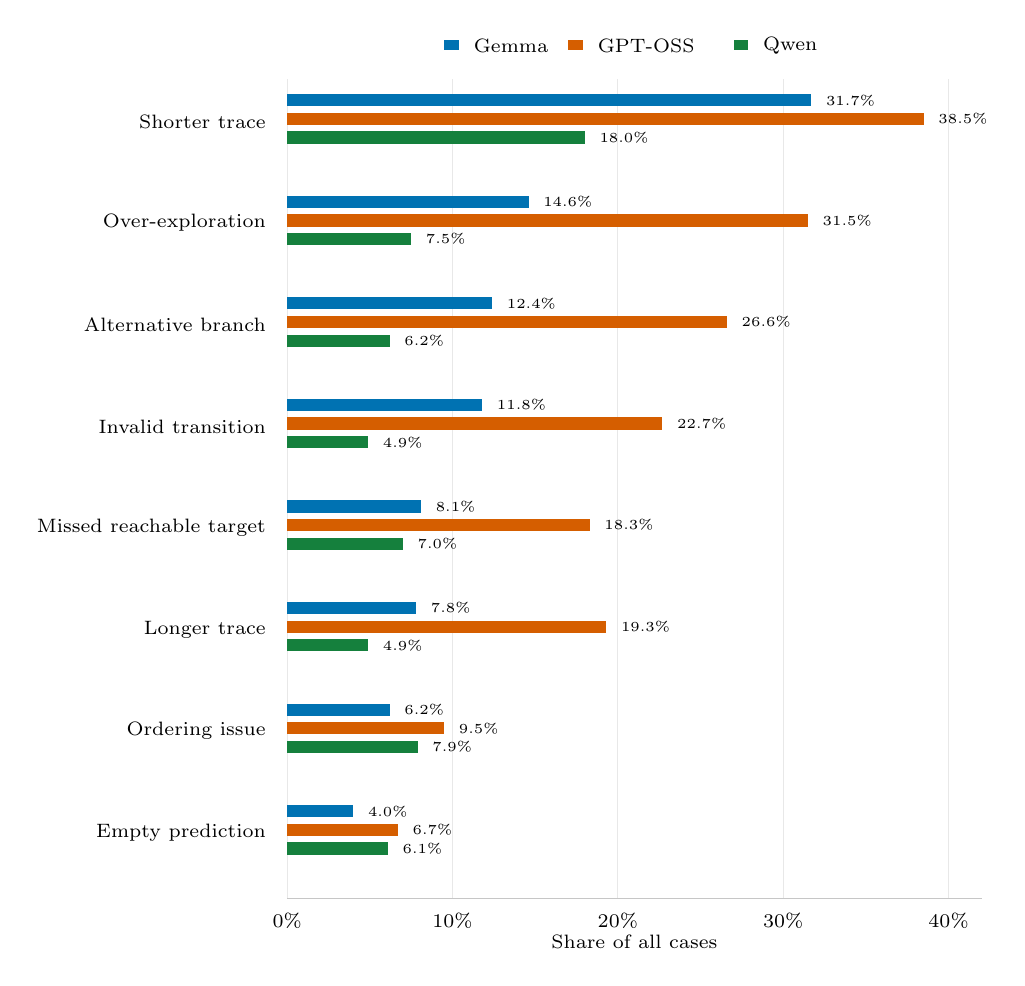
\begin{tikzpicture}[x=0.21cm,y=0.43cm]
        \foreach \x/\lab in {0/0\%,10/10\%,20/20\%,30/30\%,40/40\%} {
            \draw[gray!18] (\x,0) -- (\x,24.2);
            \node[below,font=\scriptsize] at (\x,-0.15) {\lab};
        }
        \draw[gray!45] (0,0) -- (42,0);

        \node[anchor=east,font=\scriptsize] at (-0.7,22.95) {Shorter trace};
        \fill[modelblue] (0,23.40) rectangle (31.7,23.76);
        \node[right,font=\tiny] at (32.0,23.58) {31.7\%};
        \fill[modelorange] (0,22.85) rectangle (38.5,23.21);
        \node[right,font=\tiny] at (38.8,23.03) {38.5\%};
        \fill[modelgreen] (0,22.30) rectangle (18.0,22.66);
        \node[right,font=\tiny] at (18.3,22.48) {18.0\%};

        \node[anchor=east,font=\scriptsize] at (-0.7,19.95) {Over-exploration};
        \fill[modelblue] (0,20.40) rectangle (14.6,20.76);
        \node[right,font=\tiny] at (14.9,20.58) {14.6\%};
        \fill[modelorange] (0,19.85) rectangle (31.5,20.21);
        \node[right,font=\tiny] at (31.8,20.03) {31.5\%};
        \fill[modelgreen] (0,19.30) rectangle (7.5,19.66);
        \node[right,font=\tiny] at (7.8,19.48) {7.5\%};

        \node[anchor=east,font=\scriptsize] at (-0.7,16.95) {Alternative branch};
        \fill[modelblue] (0,17.40) rectangle (12.4,17.76);
        \node[right,font=\tiny] at (12.7,17.58) {12.4\%};
        \fill[modelorange] (0,16.85) rectangle (26.6,17.21);
        \node[right,font=\tiny] at (26.9,17.03) {26.6\%};
        \fill[modelgreen] (0,16.30) rectangle (6.2,16.66);
        \node[right,font=\tiny] at (6.5,16.48) {6.2\%};

        \node[anchor=east,font=\scriptsize] at (-0.7,13.95) {Invalid transition};
        \fill[modelblue] (0,14.40) rectangle (11.8,14.76);
        \node[right,font=\tiny] at (12.1,14.58) {11.8\%};
        \fill[modelorange] (0,13.85) rectangle (22.7,14.21);
        \node[right,font=\tiny] at (23.0,14.03) {22.7\%};
        \fill[modelgreen] (0,13.30) rectangle (4.9,13.66);
        \node[right,font=\tiny] at (5.2,13.48) {4.9\%};

        \node[anchor=east,font=\scriptsize] at (-0.7,10.95) {Missed reachable target};
        \fill[modelblue] (0,11.40) rectangle (8.1,11.76);
        \node[right,font=\tiny] at (8.4,11.58) {8.1\%};
        \fill[modelorange] (0,10.85) rectangle (18.3,11.21);
        \node[right,font=\tiny] at (18.6,11.03) {18.3\%};
        \fill[modelgreen] (0,10.30) rectangle (7.0,10.66);
        \node[right,font=\tiny] at (7.3,10.48) {7.0\%};

        \node[anchor=east,font=\scriptsize] at (-0.7,7.95) {Longer trace};
        \fill[modelblue] (0,8.40) rectangle (7.8,8.76);
        \node[right,font=\tiny] at (8.1,8.58) {7.8\%};
        \fill[modelorange] (0,7.85) rectangle (19.3,8.21);
        \node[right,font=\tiny] at (19.6,8.03) {19.3\%};
        \fill[modelgreen] (0,7.30) rectangle (4.9,7.66);
        \node[right,font=\tiny] at (5.2,7.48) {4.9\%};

        \node[anchor=east,font=\scriptsize] at (-0.7,4.95) {Ordering issue};
        \fill[modelblue] (0,5.40) rectangle (6.2,5.76);
        \node[right,font=\tiny] at (6.5,5.58) {6.2\%};
        \fill[modelorange] (0,4.85) rectangle (9.5,5.21);
        \node[right,font=\tiny] at (9.8,5.03) {9.5\%};
        \fill[modelgreen] (0,4.30) rectangle (7.9,4.66);
        \node[right,font=\tiny] at (8.2,4.48) {7.9\%};

        \node[anchor=east,font=\scriptsize] at (-0.7,1.95) {Empty prediction};
        \fill[modelblue] (0,2.40) rectangle (4.0,2.76);
        \node[right,font=\tiny] at (4.3,2.58) {4.0\%};
        \fill[modelorange] (0,1.85) rectangle (6.7,2.21);
        \node[right,font=\tiny] at (7.0,2.03) {6.7\%};
        \fill[modelgreen] (0,1.30) rectangle (6.1,1.66);
        \node[right,font=\tiny] at (6.4,1.48) {6.1\%};

        \fill[modelblue] (9.5,25.05) rectangle ++(0.9,0.30);
        \node[right,font=\scriptsize] at (10.7,25.20) {Gemma};
        \fill[modelorange] (17.0,25.05) rectangle ++(0.9,0.30);
        \node[right,font=\scriptsize] at (18.2,25.20) {GPT-OSS};
        \fill[modelgreen] (27.0,25.05) rectangle ++(0.9,0.30);
        \node[right,font=\scriptsize] at (28.2,25.20) {Qwen};
        \node[below,font=\scriptsize] at (21,-0.80) {Share of all cases};
    \end{tikzpicture}
    \caption{Dominant failure families from the in-depth analysis for chain-level errors. Families are normalized by all evaluated cases and are not mutually exclusive, because a single trace can expose several local characteristics.}
    \Description{Grouped horizontal LaTeX bar chart of aggregated failure families for the three models.}
    \label{fig:error-taxonomy-latex}
\end{figure*}

\begin{table*}[!t]
\centering
\caption{Planned error-family taxonomy. Counts remain TODOs until final reruns and dashboard inspection are complete.}
\label{tab:error-taxonomy}
\tiny
\setlength{\tabcolsep}{2pt}
\begin{tabularx}{\textwidth}{p{0.15\textwidth}p{0.27\textwidth}p{0.21\textwidth}p{0.055\textwidth}p{0.055\textwidth}p{0.15\textwidth}}
\toprule
Error family & Definition & Detection method & $n$ & \% & Example \\
\midrule
Syntactic-call bias & Follows a visible call that is not executable under generated guards. & Compare predicted edges with executable graph. & \TODO{n} & \TODO{\%} & false guarded call \\
Missing intermediate nodes & Skips one or more oracle methods. & Trace alignment. & \TODO{n} & \TODO{\%} & $A,C$ for $A,B,C$ \\
Early stopping & Ends before oracle exploration is complete. & Prefix and coverage checks. & \TODO{n} & \TODO{\%} & source only \\
Over-exploration & Adds reachable but non-oracle exploration after the stopping point. & Oracle stop-condition check. & \TODO{n} & \TODO{\%} & past target \\
Invalid transition & Predicts an edge absent from the executable graph. & Edge-validity check. & \TODO{n} & \TODO{\%} & cross branch \\
Target hallucination & Mentions a target or method name not present in the generated class. & Method-list check. & \TODO{n} & \TODO{\%} & unknown name \\
Positive shortcut & Gives a reachable label with a shortest-path-like trace that omits required exploration. & Canonical-trace comparison. & \TODO{n} & \TODO{\%} & path only \\
Negative over-exploration & Negative trace explores outside the source-reachable region. & Reachable-region check. & \TODO{n} & \TODO{\%} & sibling subtree \\
Wrong source & Starts the trace from a method other than the queried source. & First-node check. & \TODO{n} & \TODO{\%} & target first \\
Repeated methods & Repeats methods in an acyclic tree trace. & Duplicate check. & \TODO{n} & \TODO{\%} & $A,B,A$ \\
Order violation & Uses valid methods but not in canonical order. & Ordered oracle comparison. & \TODO{n} & \TODO{\%} & sibling swap \\
Invalid JSON / schema failure & Output cannot be parsed into the required schema. & Parser status. & \TODO{n} & \TODO{\%} & missing field \\
\bottomrule
\end{tabularx}
\end{table*}

\begin{table*}[t]
    \centering
    \caption{Evolution of dominant chain-level failure families across requested reasoning budgets. Rates are percentages of all cases for the corresponding model and budget. Families are derived from deeper-analysis tags: shorter traces use \texttt{length\_shorter}, over-exploration uses \texttt{extra\_known\_internal} or \texttt{extra\_known\_leaf}, alternative branches use \texttt{coverage\_overlap}, invalid transitions use \texttt{structure\_with\_jump}, and missed reachable targets use \texttt{target\_expected\_missing}.}
    \label{tab:failure-budget-evolution}
    \scriptsize
    \begin{tabular}{llrrrrrr}
        \toprule
        Model & Failure family & 512 & 1k & 2k & 4k & 8k & 16k \\
        \midrule
        Gemma & Shorter trace & 32.2 & 31.9 & 30.9 & 31.7 & 31.1 & 32.3 \\
        Gemma & Over-exploration & 13.6 & 14.0 & 14.1 & 14.8 & 15.3 & 14.9 \\
        Gemma & Alternative branch & 12.1 & 12.1 & 11.8 & 12.7 & 12.9 & 12.8 \\
        Gemma & Invalid transition & 10.1 & 10.7 & 11.4 & 12.3 & 12.9 & 12.5 \\
        Gemma & Reachable target missed & 9.8 & 8.6 & 8.0 & 7.9 & 7.1 & 7.5 \\
        \midrule
        GPT-OSS & Shorter trace & 39.8 & 37.7 & 35.1 & 38.0 & 39.8 & 40.9 \\
        GPT-OSS & Over-exploration & 37.1 & 33.1 & 27.8 & 22.9 & 22.1 & 21.7 \\
        GPT-OSS & Alternative branch & 42.4 & 35.5 & 26.6 & 20.3 & 18.1 & 16.5 \\
        GPT-OSS & Invalid transition & 27.9 & 23.1 & 18.6 & 15.8 & 13.8 & 13.0 \\
        GPT-OSS & Reachable target missed & 28.8 & 24.9 & 18.5 & 14.1 & 12.1 & 11.2 \\
        \midrule
        Qwen & Shorter trace & 29.6 & 25.7 & 18.6 & 12.2 & 10.4 & 11.4 \\
        Qwen & Over-exploration & 15.7 & 10.5 & 5.9 & 3.1 & 1.5 & 1.4 \\
        Qwen & Alternative branch & 14.8 & 10.2 & 6.0 & 3.0 & 1.5 & 1.5 \\
        Qwen & Invalid transition & 9.2 & 5.2 & 3.9 & 2.4 & 1.1 & 1.2 \\
        Qwen & Reachable target missed & 16.6 & 12.3 & 7.1 & 3.4 & 1.5 & 1.0 \\
        \bottomrule
    \end{tabular}
\end{table*}

\begin{table*}[t]
    \centering
    \caption{Representative local motifs for the deeper-analysis failure families. Notation: \texttt{S}=source, \texttt{T}=target, \texttt{B}=node present in both reference and prediction, \texttt{E}=reference-only node, \texttt{P}=prediction-only node. Motifs compact recurring local-graph signatures rather than individual examples.}
    \label{tab:local-motif-examples}
    \small
    \begin{tabularx}{\textwidth}{p{0.20\textwidth}p{0.25\textwidth}X}
        \toprule
        Failure family & Example local motif & Interpretation \\
        \midrule
        Shorter trace & \texttt{S -> B -> B; B -> E -> ...} & The prediction follows a valid prefix and then stops before the reference suffix. \\
        Over-exploration & \texttt{S -> B -> P -> P} & The model keeps traversing prediction-only nodes after leaving the reference path. \\
        Alternative branch & \texttt{B -> E; B -> P} & The prediction shares a prefix, then chooses a sibling or nearby branch instead of the oracle branch. \\
        Invalid transition & \texttt{B -> P} with no graph edge & The predicted transition is not a valid local call edge. \\
        Reachable target missed & \texttt{S -> B -> E -> T} & The target is reachable in the oracle trace, but the predicted trace omits the target-bearing suffix. \\
        Longer trace & \texttt{S -> B -> T -> P} & The prediction reaches the relevant region but continues beyond the reference trace. \\
        Order issue & \texttt{S -> B1, S -> B2} with swapped visits & The local calls are plausible, but the traversal order disagrees with the reference order. \\
        Empty prediction & \texttt{S -> E, S -> E} & The reference has reachable outgoing structure, but the extracted prediction is empty. \\
        Hallucinated target & \texttt{B -> P -> T} & The prediction reaches the target through a prediction-only suffix absent from the oracle path. \\
        Target at wrong rank & \texttt{S -> T -> B} vs. \texttt{S -> B -> T} & The target appears, but at the wrong position in the traversal. \\
        Repeated methods & \texttt{B -> P -> P} & A method or occurrence is repeated in the prediction without a matching repetition in the oracle trace. \\
        Unresolved node & \texttt{B -> P(unresolved)} & The prediction introduces a method name that cannot be resolved in the parsed call graph. \\
        Wrong source & \texttt{P -> P; S -> E} & The predicted trace starts from a node other than the required source anchor. \\
        \bottomrule
    \end{tabularx}
\end{table*}

\begin{table*}[t]
    \centering
    \caption{Example of a correct final answer with an incorrect trace. The target is reachable, but the model skips the intermediate method, so final-answer accuracy overestimates path fidelity.}
    \label{tab:example}
    \small
    \begin{tabularx}{\textwidth}{p{0.17\textwidth}X}
        \toprule
        Field & Value \\
        \midrule
        Question & Does `loadValueFromDatabase` call `calculateMetricInThread`, directly or indirectly? \\
        Budget / depth & 512 tokens / depth 2 \\
        Oracle chain & \texttt{loadValueFromDatabase} \(\rightarrow\) \texttt{dispatchEventForExecution} \(\rightarrow\) \texttt{calculateMetricInThread} \\
        Predicted trace & \texttt{loadValueFromDatabase} \(\rightarrow\) \texttt{calculateMetricInThread} \\
        Interpretation & The final answer is \true, but the reasoning trace contains a shortcut edge that is not present in the oracle call path. \\
        \bottomrule
    \end{tabularx}
\end{table*}

\begin{table*}[t]
    \centering
    \caption{Preliminary contrasts between factors on the shared slice. Values are deltas in percentage points between stressed and baseline conditions, computed by comparing the highest indicated distractor level to the lowest while aggregating over the shared model/context/depth/budget slice. These are descriptive contrasts, not adjusted causal estimates.}
    \label{tab:factors}
    \small
    \begin{tabular}{l rr rr rr}
        \toprule
        & \multicolumn{2}{c}{Gemma} & \multicolumn{2}{c}{GPT-OSS} & \multicolumn{2}{c}{Qwen} \\
        \cmidrule(lr){2-3}\cmidrule(lr){4-5}\cmidrule(lr){6-7}
        Factor contrast & Final & Chain & Final & Chain & Final & Chain \\
        \midrule
        comment: 0 -> 1 & -6.7 pp & -10.5 pp & -6.4 pp & -7.2 pp & -2.2 pp & -4.0 pp \\
        variable: 0 -> 2 & -5.1 pp & -8.1 pp & -4.5 pp & -5.0 pp & -2.4 pp & -3.9 pp \\
        loop: 0 -> 3 & -3.6 pp & -8.5 pp & -7.6 pp & -8.2 pp & -2.0 pp & -5.0 pp \\
        if: 1 -> 2 & -3.6 pp & -9.5 pp & -7.5 pp & -8.3 pp & -2.4 pp & -6.1 pp \\
        parameter: 0 -> 2 & -2.4 pp & -3.2 pp & -1.9 pp & -2.4 pp & -0.8 pp & +0.8 pp \\
        \bottomrule
    \end{tabular}
\end{table*}


\begin{itemize}[leftmargin=*]
    \item Use these figures and tables to support the analysis of trace fidelity, failure modes, and budget sensitivity in \researchq{4}.
\end{itemize}

\section{Error Analysis}
\label{sec:error-analysis}

Beyond aggregate metrics, we conduct a semi-quantitative error analysis with an interactive dashboard that groups trace failures by structural parameters, model configuration, reasoning-budget setting when applicable, and local graph motifs. This analysis identifies recurrent error families, including syntactic-call bias in condition-aware instances, where models follow visible but non-executable calls.

\begin{figure}[t]
\centering
\resizebox{\columnwidth}{!}{%
\begin{tikzpicture}[
    >=Latex,
    method/.style={rb method, minimum width=1.0cm},
    code/.style={rb code, text width=4.7cm},
    edge/.style={rb edge},
    bad/.style={rb optional edge, line width=1pt}
]
\node[method] (a) at (0,0) {A};
\node[method] (b) at (-1.2,-1.0) {B};
\node[method] (c) at (1.2,-1.0) {C};
\draw[edge] (a) -- node[left, font=\scriptsize] {true branch} (b);
\draw[bad] (a) -- node[right, font=\scriptsize] {false branch} (c);
\node[code, right=2.1cm of a] (snippet) {
\texttt{void A() \{}\\
\quad \texttt{if (x > 0) B();}\\
\quad \texttt{if (x < 0) C();}\\
\texttt{\}}\\
\texttt{// generated x = 1}
};
\end{tikzpicture}
}
\caption{Schematic syntactic-call bias. A call to \texttt{C} is visible in the source code, but the generated condition is false, so \texttt{C} is excluded from the executable call graph and oracle trace.}
\Description{A small call-graph and code schematic showing a true guarded call and a false guarded call.}
\label{fig:syntactic-call-bias}
\end{figure}

\begin{table*}[!t]
\centering
\caption{Planned error-family taxonomy. Counts remain TODOs until final reruns and dashboard inspection are complete.}
\label{tab:error-taxonomy}
\tiny
\setlength{\tabcolsep}{2pt}
\begin{tabularx}{\textwidth}{p{0.15\textwidth}p{0.27\textwidth}p{0.21\textwidth}p{0.055\textwidth}p{0.055\textwidth}p{0.15\textwidth}}
\toprule
Error family & Definition & Detection method & $n$ & \% & Example \\
\midrule
Syntactic-call bias & Follows a visible call that is not executable under generated guards. & Compare predicted edges with executable graph. & \TODO{n} & \TODO{\%} & false guarded call \\
Missing intermediate nodes & Skips one or more oracle methods. & Trace alignment. & \TODO{n} & \TODO{\%} & $A,C$ for $A,B,C$ \\
Early stopping & Ends before oracle exploration is complete. & Prefix and coverage checks. & \TODO{n} & \TODO{\%} & source only \\
Over-exploration & Adds reachable but non-oracle exploration after the stopping point. & Oracle stop-condition check. & \TODO{n} & \TODO{\%} & past target \\
Invalid transition & Predicts an edge absent from the executable graph. & Edge-validity check. & \TODO{n} & \TODO{\%} & cross branch \\
Target hallucination & Mentions a target or method name not present in the generated class. & Method-list check. & \TODO{n} & \TODO{\%} & unknown name \\
Positive shortcut & Gives a reachable label with a shortest-path-like trace that omits required exploration. & Canonical-trace comparison. & \TODO{n} & \TODO{\%} & path only \\
Negative over-exploration & Negative trace explores outside the source-reachable region. & Reachable-region check. & \TODO{n} & \TODO{\%} & sibling subtree \\
Wrong source & Starts the trace from a method other than the queried source. & First-node check. & \TODO{n} & \TODO{\%} & target first \\
Repeated methods & Repeats methods in an acyclic tree trace. & Duplicate check. & \TODO{n} & \TODO{\%} & $A,B,A$ \\
Order violation & Uses valid methods but not in canonical order. & Ordered oracle comparison. & \TODO{n} & \TODO{\%} & sibling swap \\
Invalid JSON / schema failure & Output cannot be parsed into the required schema. & Parser status. & \TODO{n} & \TODO{\%} & missing field \\
\bottomrule
\end{tabularx}
\end{table*}


\TODO{Insert final counts and percentages for each error family after inspecting the final dashboard.}

The taxonomy explains mechanisms behind aggregate degradation. Syntactic-call bias tests whether condition-aware failures come from treating visible calls as executable; missing-node and shortcut errors capture answers that are correct without recovering the required execution-oriented trace. The dashboard supports this interpretation but is not the source of the primary benchmark scores. The main paper includes one representative schematic example; full screenshots and usage notes belong in the appendix or artifact documentation. \TODO{Add final deeper-analysis figure and dashboard appendix or artifact reference.}

\section{Discussion and Threats to Validity}
\label{sec:discussion}

\subsection{Construct Validity}

\benchmark measures observable answers and emitted traces for generated method-reachability questions. Trace correctness is not a direct measurement of hidden model cognition: a model may emit the right trace for the wrong reason, or answer correctly while giving an invalid path. Likewise, reasoning text from locally run models is an output artifact, not a complete record of internal computation. Reporting answer, trace, exploration, and invalid-output metrics reduces the risk of overinterpreting any single signal.

\subsection{Internal Validity}

The main internal-validity risks are generator defects, oracle mismatch, prompt ambiguity, parsing failures, and uncontrolled inference settings. The oracle-validation pipeline checks compilation, materialized call consistency, positive and negative reachability labels, canonical traces, and condition evaluation for guarded calls. Before quantitative claims are made, the final protocol must also freeze prompt templates, model identifiers, decoding parameters, and budget settings.

\TODO{Rerun all final experiments after freezing datasets, prompts, model versions, inference settings, and evaluation scripts.}

\subsection{External Validity}

\benchmark trades ecological realism for oracle labels, parameterized factors, and trace-level validation. It uses generated Java programs rather than real repositories, so it does not capture the full complexity of naming conventions, architectural patterns, dependencies, side effects, or domain semantics found in production code. The same restriction gives the benchmark its diagnostic value: individual factors can be varied while keeping the task and oracle stable.

The current benchmark targets Java and materializes each instance as a single class with many methods. It does not measure full Java comprehension, realistic project-level reasoning, inheritance, interfaces, dynamic dispatch, overloading, exceptions, recursion, external libraries, multi-class designs, cyclic call graphs, realistic naming conventions, rich data flow, arbitrary loop-guarded reachability, or human-written architecture. Current graphs are acyclic trees, and condition-aware reachability is limited to \texttt{if} statements.

The generator starts from abstract call graphs, so the core design is partly language-agnostic. Extending the benchmark to other languages would require a new materialization and validation backend, as well as language-specific prompt examples.

\benchmark isolates a lower-level structural capability that may be hidden inside broader software-engineering tasks. Its results should therefore be read as evidence about executable method reachability under controlled conditions, not as a direct estimate of performance on full maintenance workflows.

\subsection{Conclusion Validity}

Current quantitative results are preliminary. Final claims require a stabilized rerun, consistent handling of \texttt{NO\_RESPONSE}, and analyses that separate answer accuracy, trace quality, graph-valid exploration, structural-factor effects, model-configuration differences, and budget effects where controls are verified. Because the current unguarded and condition-aware datasets are not paired instance-by-instance, family comparisons should not be analyzed as paired tests unless the frozen dataset changes. Results may also be sensitive to prompt format, JSON extraction, serving configuration, decoding parameters, and model-version drift. Budget sensitivity should remain part of the model/inference-mode analysis rather than a standalone claim unless additional experiments show that it explains failures across both task families.

\subsection{Reproducibility and Artifact Availability}

Model availability, licenses, model sizes, context lengths, and reasoning-budget support are temporally unstable. The final paper must verify and cite these claims from official sources before submission. \TODO{Verify exact model identifiers, sizes, licenses, context lengths, and Jean Zay compatibility.}

The intended artifact should include datasets, generation code, prompt templates, evaluation scripts, oracle validators, and dashboard materials. During review, links must preserve double-anonymous requirements; after acceptance, public links should be made stable when possible. \TODO{Add anonymized artifact URL, artifact contents checklist, and public-release plan.}

\section{Conclusion}
\label{sec:conclusion}

This paper presents \benchmark, the final generated dataset of Java classes and method-reachability questions, together with the controlled algorithm used to construct it. Each question has a Boolean label and an executable-graph oracle, allowing decisions and supporting traces to be evaluated independently.

The evaluation shows that correct decisions often lack valid executable evidence. Conditions, passed values, and the exhaustive exploration required by negative questions produce the strongest difficulties. Trace diagnostics locate errors around disabled calls, omitted methods, and longer value dependencies.

Providing the \texttt{main} entry point and explicitly describing the deterministic execution improves the observed scores, but the difficulties with guarded value propagation remain. The main comparison also increases the reasoning budget. At a fixed budget, Qwen3.8-Flash-Next improves its trace scores on the difficult subset while producing more non-responses. These findings show why reachability should be evaluated through both decisions and executable evidence, with the prompt context made explicit. Further evaluation on more models and real programs would test how broadly these difficulties transfer.


\bibliographystyle{ACM-Reference-Format}
\bibliography{bibliography/references}

\end{document}
